%=====================================================================
%  SAR -> Optical Feature Reconstruction (arm ED)
%  A companion volume to project_explanation.tex
%  Compile with:  pdflatex encoder_decoder_explained.tex   (run twice)
%=====================================================================
\documentclass[11pt,a4paper]{report}

\usepackage[T1]{fontenc}
\usepackage[utf8]{inputenc}
\usepackage[margin=2.4cm]{geometry}
\usepackage{amsmath,amssymb}
\usepackage{booktabs}
\usepackage{longtable}
\usepackage{array}
\usepackage{graphicx}
\usepackage{xcolor}
\usepackage{tikz}
\usepackage{tcolorbox}
\usepackage{enumitem}
\usepackage{microtype}
\usepackage{caption}
\usepackage{listings}
\usepackage[hidelinks,bookmarks=true]{hyperref}

\usetikzlibrary{arrows.meta,positioning,fit,backgrounds,shapes.geometric,calc,decorations.pathreplacing}
\tcbuselibrary{skins,breakable}

%---------------------------------------------------------------- colours
\definecolor{accent}{HTML}{2A78D6}
\definecolor{warm}{HTML}{EB6834}
\definecolor{teal}{HTML}{1BAF7A}
\definecolor{plum}{HTML}{8256D0}
\definecolor{ink}{HTML}{0B0B0B}
\definecolor{soft}{HTML}{52514E}
\definecolor{rule}{HTML}{E3E3DF}
\definecolor{codebg}{HTML}{F7F7F5}

%---------------------------------------------------------------- boxes
\newtcolorbox{codedoes}[1][]{
  breakable, enhanced, colback=accent!4, colframe=accent,
  boxrule=0.4pt, left=6pt, right=6pt, top=5pt, bottom=5pt,
  fonttitle=\bfseries\small, title={What the code actually does}, #1}

\newtcolorbox{whybox}[1][]{
  breakable, enhanced, colback=teal!5, colframe=teal,
  boxrule=0.4pt, left=6pt, right=6pt, top=5pt, bottom=5pt,
  fonttitle=\bfseries\small, title={Why it was chosen (design rationale)}, #1}

\newtcolorbox{flagbox}[1][]{
  breakable, enhanced, colback=warm!6, colframe=warm,
  boxrule=0.6pt, left=6pt, right=6pt, top=5pt, bottom=5pt,
  fonttitle=\bfseries\small, title={Caveat / correction -- read this carefully}, #1}

\newtcolorbox{intuition}[1][]{
  breakable, enhanced, colback=gray!6, colframe=soft,
  boxrule=0.4pt, left=6pt, right=6pt, top=5pt, bottom=5pt,
  fonttitle=\bfseries\small, title={Intuition first}, #1}

\newtcolorbox{keyfinding}[1][]{
  breakable, enhanced, colback=plum!7, colframe=plum,
  boxrule=0.8pt, left=6pt, right=6pt, top=5pt, bottom=5pt,
  fonttitle=\bfseries\small, title={Key finding}, #1}

%---------------------------------------------------------------- code style
\lstdefinestyle{py}{
  language=Python, basicstyle=\ttfamily\footnotesize,
  backgroundcolor=\color{codebg}, frame=single, rulecolor=\color{rule},
  keywordstyle=\color{accent}, commentstyle=\color{soft}\itshape,
  stringstyle=\color{teal}, showstringspaces=false,
  breaklines=true, columns=fullflexible, xleftmargin=4pt, framexleftmargin=4pt}
\lstset{style=py}

\newcommand{\file}[1]{\texttt{\small #1}}
\newcommand{\code}[1]{\texttt{\small #1}}
\newcommand{\zc}{\mathbf{z}_{\text{clean}}}
\newcommand{\zd}{\mathbf{z}_{\text{degraded}}}
\newcommand{\zs}{\mathbf{z}_{\text{sar}}}
\newcommand{\zh}{\hat{\mathbf{z}}_{\text{clean}}}

\setlist[itemize]{itemsep=2pt,topsep=3pt}
\setlist[enumerate]{itemsep=2pt,topsep=3pt}

%=====================================================================
\begin{document}

\begin{titlepage}
\centering
\vspace*{2.0cm}
{\Huge\bfseries Can Radar Predict\\[2mm] What the Camera Would Have Seen?\par}
\vspace{0.8cm}
{\LARGE SAR $\rightarrow$ Optical Feature Reconstruction\par}
\vspace{0.4cm}
{\large\itshape An additional experiment, explained from first principles\par}
\vspace{1.8cm}

\begin{minipage}{0.86\textwidth}
\small
This is a companion volume to \file{project\_explanation.tex}. That document
covers the main study: whether Sentinel-1 radar recovers land-cover information
that cloud destroys in Sentinel-2 optical imagery, answered by concatenating the
two modalities' features.

\medskip
This document covers a \emph{different and strictly stronger} question. Rather
than asking whether radar is \emph{useful alongside} a cloud-damaged optical
image, it asks whether radar can \emph{predict the optical representation
itself} --- the numerical fingerprint a cloud-free image would have produced.

\medskip
Everything is explained from the ground up. If you know what a neural network
and a training loop are, you have enough background. No remote-sensing knowledge
is assumed.

\medskip
Every number in this document was read out of a results file, and the file and
the value are named at the point of use. Chapter~\ref{ch:verify} lists them all
in one place. The original experiment's results were not modified, re-run, or
re-tuned to accommodate this one.
\end{minipage}

\vfill
{\small Companion to \file{project\_explanation.tex} and \file{README.md} \S17\par}
\vspace{1.0cm}
\end{titlepage}

\tableofcontents
\clearpage

%=====================================================================
\chapter{The Two Questions}
\label{ch:two}

\section{What the original experiment asked}

The main study compares four arms. Stripped of detail, the interesting pair is:

\begin{itemize}
\item \textbf{Arm B} --- classify from the cloud-damaged optical image alone.
\item \textbf{Arm C} --- classify from the cloud-damaged optical image
      \emph{plus} the radar image.
\end{itemize}

If C beats B, radar carried information that helped. That is a perfectly good
question and the main document answers it carefully: at 80\% simulated cloud, in
the fair comparison, radar buys $+0.037$ macro F1, and roughly 90\% of what
naively looks like a radar benefit is actually the benefit of training on
degraded data at all.

\section{What this experiment asks instead}

Arm C uses radar the way you would use any extra input: bolt it on and let the
classifier work out what to do with it. That tests \emph{usefulness}.

This document tests \emph{substitutability}:

\begin{quote}\itshape
Can Sentinel-1 radar predict the optical representation that a cloud-free
Sentinel-2 image would have produced?
\end{quote}

\begin{intuition}
The difference matters, and it is easy to miss.

\medskip
Suppose you are describing a landscape to someone over the phone, and your view
is fogged. A friend standing next to you has a thermal camera. Two ways they can
help:

\medskip
\textbf{The arm C way.} They read out their thermal readings, you read out what
you can still see, and the person on the other end combines both. They need no
shared vocabulary --- the listener does the work.

\medskip
\textbf{The arm ED way.} Your friend uses their thermal readings to
\emph{guess what you would have seen} if the fog lifted, and reports that
instead. Now they must speak your language: their output has to be a
plausible visual description, not a temperature reading.

\medskip
The second is harder, and it can fail in a way the first cannot: the thermal
camera might carry real information that simply has no visual equivalent.
\end{intuition}

These two can come apart in both directions:

\begin{itemize}
\item Radar could \emph{help a classifier} while being a \emph{poor predictor}
      of optical features --- it contributes information in its own coordinate
      system that has no optical analogue.
\item Radar could \emph{predict optical features well} while adding
      \emph{nothing a classifier can use} --- it only recovers the parts of the
      optical representation the surviving pixels already provided.
\end{itemize}

Because neither implies the other, this is run as a genuinely separate arm and
measured on its own terms, not inferred from the arm C result.

\begin{flagbox}
\textbf{What is \emph{not} being reconstructed.} This never reconstructs
Sentinel-2 \emph{pixels}. It reconstructs the 384-number feature vector the
Vision Transformer produces. If you take one thing from this chapter, take that.
The distinction is the subject of Chapter~\ref{ch:features}, and every claim in
this document depends on it.
\end{flagbox}

\section{Naming}

To keep the two experiments distinct, this arm is called \textbf{ED}
(encoder--decoder), and its two training regimes are \textbf{ED-R1} and
\textbf{ED-R2}, mirroring R1 and R2 in the main study. These names never mix.

\begin{center}
\small
\begin{tabular}{@{}llp{7.6cm}@{}}
\toprule
\textbf{Arm} & \textbf{Input to the classifier} & \textbf{Question it answers} \\
\midrule
B  & $\zd$ (384) & How much does cloud cost? \\
C  & $[\zd\,;\,\zs]$ (2432) & Is radar \emph{useful} alongside optical? \\
ED & $[\zd\,;\,\zh]$ (768) & Can radar \emph{predict} clean optical? \\
D  & $\zs$ (2048) & How good is radar on its own? \\
\bottomrule
\end{tabular}
\end{center}

%=====================================================================
\chapter{What a ``Feature'' Actually Is}
\label{ch:features}

This chapter exists because the entire experiment is a statement about feature
vectors, and the most common way to misunderstand the results is to picture
images where there are none.

\section{The network does not give you a picture back}

Feed a $12 \times 120 \times 120$ Sentinel-2 patch into the frozen Vision
Transformer and what comes out is not an image. It is a list of
\textbf{384 numbers}.

\begin{center}
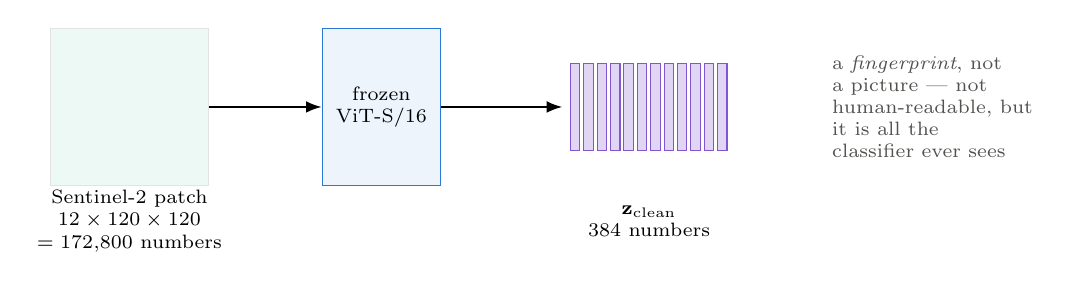
\begin{tikzpicture}[scale=1.0]
\node[draw=rule,fill=teal!8,minimum width=2.0cm,minimum height=2.0cm] (img) at (0,0) {};
\node[font=\scriptsize,align=center] at (0,-1.45) {Sentinel-2 patch\\$12\times120\times120$\\$=172{,}800$ numbers};
\node[draw=accent,fill=accent!8,minimum width=1.5cm,minimum height=2.0cm,align=center,font=\scriptsize] (vit) at (3.2,0) {frozen\\ViT-S/16};
\draw[-{Latex[length=2mm]},thick] (img) -- (vit);
\foreach \i in {0,...,11}
  \draw[fill=plum!25,draw=plum] (5.6+\i*0.17,-0.55) rectangle (5.72+\i*0.17,0.55);
\node[font=\scriptsize,align=center] at (6.6,-1.45) {$\zc$\\384 numbers};
\draw[-{Latex[length=2mm]},thick] (vit) -- (5.5,0);
\node[font=\scriptsize,soft,align=left] at (10.2,0)
  {a \emph{fingerprint}, not\\a picture --- not\\human-readable, but\\it is all the\\classifier ever sees};
\end{tikzpicture}
\end{center}

\begin{intuition}
Think of it as a fingerprint. You cannot look at a fingerprint and see a face.
But two photographs of the same person produce similar fingerprints, and
photographs of different people produce different ones. That is all a feature
vector is: a compressed identity code, useful for comparison, useless for
viewing.

\medskip
The compression here is dramatic: 172{,}800 numbers down to 384, a factor of
450. Almost everything is discarded. What survives is whatever the
self-supervised pretraining decided was worth keeping.
\end{intuition}

\section{Three feature vectors, and keeping them straight}

Everything that follows involves exactly three 384-dimensional vectors per
patch, plus one 2048-dimensional radar vector. Confusing them is the main way to
misread the experiment, so they get explicit notation.

\begin{center}
\small
\begin{tabular}{@{}llp{8.2cm}@{}}
\toprule
\textbf{Symbol} & \textbf{Dim} & \textbf{What it is} \\
\midrule
$\zc$   & 384 & Feature of the \emph{cloud-free} image. Available only in
                training. The regression target. \\
$\zd$   & 384 & Feature of the \emph{cloud-damaged} image. Available at test
                time. What arm B classifies from. \\
$\zs$   & 2048 & Feature of the radar image. Always available --- radar is never
                masked. \\
$\zh$   & 384 & The decoder's \emph{estimate} of $\zc$, computed from $\zs$
                alone. The hat means \emph{guess}. \\
\bottomrule
\end{tabular}
\end{center}

\begin{flagbox}
$\zh$ is \textbf{not} $\zc$. The hat is not decoration. $\zc$ is the truth and is
unavailable at test time; $\zh$ is a prediction made without it. Chapter
\ref{ch:leak} verifies that the code cannot confuse the two even by accident.
\end{flagbox}

\section{How far does cloud move the feature?}

Before asking whether radar can repair the feature, it is worth knowing how
badly cloud damages it. Masking 80\% of the image moves the optical feature by a
relative $L_2$ distance of $0.421$ --- the damaged fingerprint sits 42\% of its
own length away from the clean one.

\begin{codedoes}
Measured directly from the cached features:
\begin{lstlisting}
c = np.load('data/features/train_opt_L000.npy')   # z_clean
d = np.load('data/features/train_opt_L080.npy')   # z_degraded at 80%
np.linalg.norm(c - d, axis=1).mean() / np.linalg.norm(c, axis=1).mean()
# -> 0.421
\end{lstlisting}
Mean feature norm $\|\zc\| = 9.50$; mean radar feature norm is $43.73$ on the
training split.
\end{codedoes}

That $0.421$ is the gap the decoder is being asked to close.

%=====================================================================
\chapter{The Architecture}
\label{ch:arch}

\section{The whole thing in one diagram}

\begin{center}
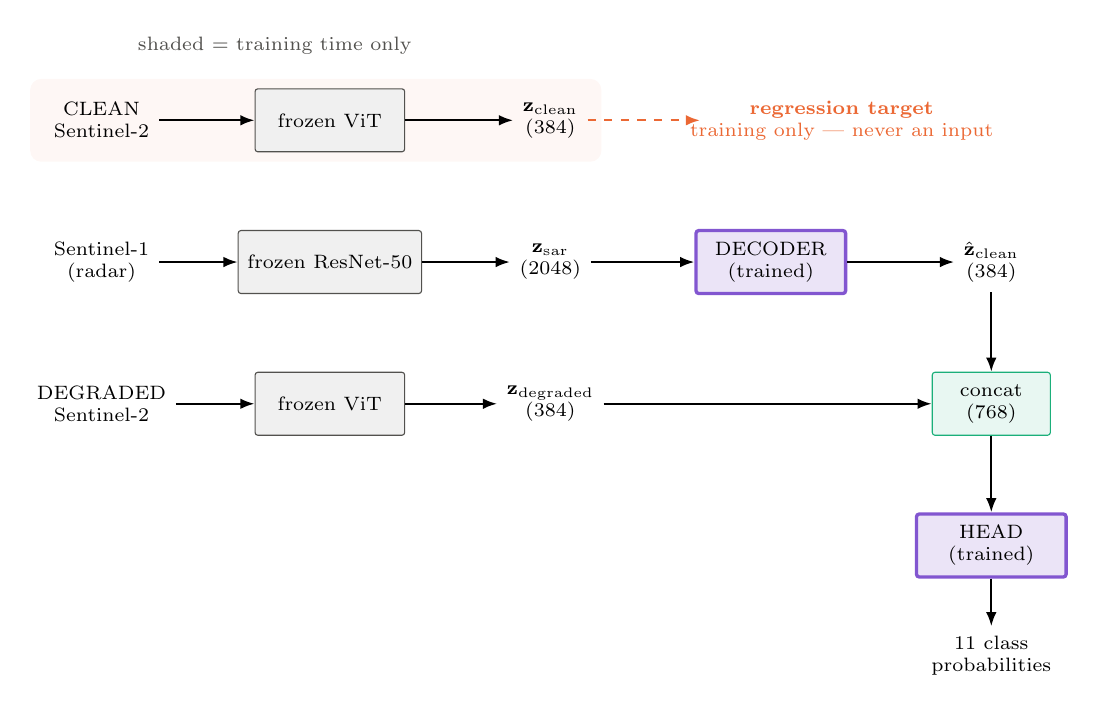
\begin{tikzpicture}[
  box/.style={draw=rule,rounded corners=1pt,minimum height=8mm,font=\scriptsize,align=center},
  enc/.style={box,fill=accent!10,draw=accent,minimum width=1.9cm},
  frz/.style={box,fill=gray!12,draw=soft,minimum width=1.9cm},
  trn/.style={box,fill=plum!16,draw=plum,minimum width=1.9cm,very thick},
  vec/.style={font=\scriptsize,align=center},
  ar/.style={-{Latex[length=1.8mm]},thick},
]
% row 1: clean, training only
\node[vec] (c1) at (0,3.2) {CLEAN\\Sentinel-2};
\node[frz] (v1) at (2.9,3.2) {frozen ViT};
\node[vec] (z1) at (5.7,3.2) {$\zc$\\(384)};
\draw[ar] (c1)--(v1); \draw[ar] (v1)--(z1);
\node[font=\scriptsize,warm,align=center] at (9.4,3.2)
  {\textbf{regression target}\\training only --- never an input};
\draw[ar,warm,dashed] (z1) -- (7.6,3.2);

% row 2: sar
\node[vec] (s1) at (0,1.4) {Sentinel-1\\(radar)};
\node[frz] (r1) at (2.9,1.4) {frozen ResNet-50};
\node[vec] (z2) at (5.7,1.4) {$\zs$\\(2048)};
\node[trn] (dec) at (8.5,1.4) {DECODER\\(trained)};
\node[vec] (z3) at (11.3,1.4) {$\zh$\\(384)};
\draw[ar] (s1)--(r1); \draw[ar] (r1)--(z2); \draw[ar] (z2)--(dec); \draw[ar] (dec)--(z3);

% row 3: degraded
\node[vec] (c2) at (0,-0.4) {DEGRADED\\Sentinel-2};
\node[frz] (v2) at (2.9,-0.4) {frozen ViT};
\node[vec] (z4) at (5.7,-0.4) {$\zd$\\(384)};
\draw[ar] (c2)--(v2); \draw[ar] (v2)--(z4);

% concat + head
\node[box,fill=teal!10,draw=teal,minimum width=1.5cm] (cat) at (11.3,-0.4) {concat\\(768)};
\draw[ar] (z4) -- (cat);
\draw[ar] (z3) -- (cat);
\node[trn] (head) at (11.3,-2.2) {HEAD\\(trained)};
\node[vec] (out) at (11.3,-3.6) {11 class\\probabilities};
\draw[ar] (cat)--(head); \draw[ar] (head)--(out);

\begin{scope}[on background layer]
\node[fill=warm!5,rounded corners,fit=(c1)(z1),inner sep=5pt] {};
\end{scope}
\node[font=\scriptsize,soft] at (2.2,4.15) {shaded = training time only};
\end{tikzpicture}
\end{center}

Two components are trained, shown in purple. Everything else is frozen.

\section{The decoder}

\begin{center}
\small
\begin{tabular}{@{}lll@{}}
\toprule
\textbf{Layer} & \textbf{Shape in $\rightarrow$ out} & \textbf{Why} \\
\midrule
LayerNorm & $2048 \rightarrow 2048$ & see the caveat below \\
Linear & $2048 \rightarrow 512$ & compress \\
ReLU & --- & non-linearity \\
Dropout(0.3) & --- & regularise; 4205 training patches is not many \\
Linear & $512 \rightarrow 384$ & emit an optical-shaped vector \\
\bottomrule
\end{tabular}
\end{center}

\begin{whybox}
\textbf{Why such a small network?} The experiment tests whether the mapping
$\zs \rightarrow \zc$ \emph{exists at all}. A transformer decoder here would
confound ``radar predicts optical features'' with ``a bigger network fits
better'', which is precisely the ambiguity the frozen-encoder design elsewhere in
this project exists to avoid.
\end{whybox}

\begin{flagbox}
\textbf{The input LayerNorm is a deliberate addition, and here is the evidence
for it.} The SSL4EO ResNet-50 features have mean $L_2$ norm \textbf{43.73 on the
training split but 23.95 on test}. That is a large scale shift between splits.
Without normalisation the first linear layer would bake in a magnitude the test
split does not share. Set \code{encoder\_decoder.input\_norm: false} in
\file{configs/config.yaml} to reproduce the strictly minimal MLP.

\medskip
This is an engineering judgement, not a measured result --- I did not run the
ablation with and without it.
\end{flagbox}

\section{The classifier head}

\begin{center}
\small
\begin{tabular}{@{}ll@{}}
\toprule
\textbf{Layer} & \textbf{Shape} \\
\midrule
LayerNorm & $768 \rightarrow 768$ \\
Linear & $768 \rightarrow 512$ \\
ReLU + Dropout(0.3) & --- \\
Linear & $512 \rightarrow 11$ \\
\bottomrule
\end{tabular}
\end{center}

\begin{whybox}
\textbf{Why hidden width 512 and not something bespoke?} Because arms B and C use
512, and the whole logic of the arm comparison is that every arm shares an
identical head topology and training recipe so that \emph{the only difference is
what is fed in}. Giving ED a different head would reintroduce exactly the
capacity confound the study is built to exclude.

\medskip
Configurable via \code{encoder\_decoder.head\_hidden\_dim}; \code{null} inherits the
project's 512.
\end{whybox}

\section{Every tensor, end to end}

\begin{center}
\small
\begin{tabular}{@{}llr@{}}
\toprule
\textbf{Stage} & \textbf{Tensor} & \textbf{Shape} \\
\midrule
Raw optical patch & Sentinel-2 L2A, 12 bands & $(N, 12, 120, 120)$ \\
Resized for the ViT & bilinear & $(N, 12, 224, 224)$ \\
Optical feature & $\zc$ or $\zd$ & $(N, 384)$ \\
\midrule
Raw radar patch & Sentinel-1 GRD, VV/VH & $(N, 2, 120, 120)$ \\
Resized for the ResNet & bilinear & $(N, 2, 224, 224)$ \\
Radar feature & $\zs$ & $(N, 2048)$ \\
\midrule
Decoder output & $\zh$ & $(N, 384)$ \\
Concatenated & $[\zd\,;\,\zh]$ & $(N, 768)$ \\
Logits & --- & $(N, 11)$ \\
Probabilities & after sigmoid & $(N, 11)$ \\
\bottomrule
\end{tabular}
\end{center}

With $N = 4205$ training, $2418$ validation, $2151$ test patches.

%=====================================================================
\chapter{Training, in Two Deliberately Separate Stages}
\label{ch:train}

\section{Stage 1 --- fit the decoder, with no labels at all}

The decoder is trained on one job: given $\zs$, output something close to $\zc$.

\[
\mathcal{L}_{\text{recon}} \;=\; \frac{1}{384}\,
\bigl\lVert \zh - \zc \bigr\rVert_2^2
\qquad\text{(plain mean squared error)}
\]

\begin{codedoes}
From \file{src/encoder\_decoder.py}, \code{train\_decoder()}. Model selection is
on \emph{validation reconstruction loss}, and \textbf{no class label is
touched anywhere in this function}. Optimiser AdamW, lr $10^{-3}$, weight decay
$10^{-4}$, batch 256, up to 60 epochs, early stopping after 10 without
improvement.
\end{codedoes}

\begin{whybox}
\textbf{Why keep the decoder label-free?} So that the reconstruction metrics in
Chapter~\ref{ch:recon} mean what they say. If the decoder saw labels, a good
reconstruction score would only tell you the features had been shaped for this
particular classifier --- it would stop being independent evidence that radar
predicts optical structure.
\end{whybox}

\section{Stage 2 --- freeze the decoder, train the head}

The decoder is then frozen (\code{requires\_grad\_(False)}) and the classifier
is trained on $[\zd\,;\,\zh]$ with binary cross-entropy:

\[
\mathcal{L}_{\text{cls}} = -\frac{1}{11}\sum_{k=1}^{11}
\Bigl[ y_k \log \sigma(\ell_k) + (1-y_k)\log\bigl(1-\sigma(\ell_k)\bigr) \Bigr]
\]

Sigmoid rather than softmax because this is multi-label: a patch genuinely
contains several land-cover types at once (3.5 on average), so the classes must
not compete for probability mass.

\begin{flagbox}
\textbf{Two-stage is a real limitation, and it was chosen knowingly.}
Training the decoder and head jointly end to end would almost certainly score
higher --- the decoder could shape its output for the classifier instead of for
reconstruction fidelity.

\medskip
It was rejected because a jointly-trained decoder is simply a reparameterised
fusion head. The reconstruction metric would become circular, and the
distinction this whole document rests on --- prediction versus usefulness ---
would collapse. \textbf{ED is therefore not the strongest possible version of
this idea.} It is the version that can be measured.
\end{flagbox}

\section{Regimes: ED-R1 and ED-R2}

\begin{center}
\small
\begin{tabular}{@{}lp{10.5cm}@{}}
\toprule
\textbf{ED-R1} & Head trained at 0\% masking only. Mirrors R1 --- a model that
has never seen a cloud. \\
\textbf{ED-R2} & Head trained with masking sampled per patch per epoch from
$\{0, 0.2, 0.4, 0.6, 0.8\}$. Mirrors R2. This is the fair comparison. \\
\bottomrule
\end{tabular}
\end{center}

\begin{intuition}
\textbf{The decoder is the same object in both regimes, and that is not an
oversight.} Its input is radar, which is never masked. Its target is the clean
optical feature, which by definition has no masking. So neither end of the
decoder depends on the masking level --- one decoder per seed serves both
regimes. Only the \emph{head} differs.
\end{intuition}

\section{Cost}

Because both encoders are frozen, their outputs were cached once by the main
study and reused here. The entire ED experiment --- two regimes, three variants,
three seeds --- takes \textbf{53 seconds}. The 10-seed matched comparison in
Chapter~\ref{ch:cls} takes 203 seconds.

%=====================================================================
\chapter{The Measurement Trap}
\label{ch:trap}

This is the most important chapter in the document. It is where the obvious way
to score the experiment turns out to be badly misleading, and where the result
would have been overstated by a wide margin had the control not been run.

\section{The number that looks like success}

The natural way to ask ``is $\zh$ close to $\zc$?'' is cosine similarity: 1.0
means the vectors point in exactly the same direction, 0.0 means unrelated.

\begin{center}
\Large
$\cos(\zh, \zc) = 0.9871$
\end{center}

That looks like a near-perfect reconstruction. It is not. It is very close to
meaningless.

\section{Why it is meaningless: the space is anisotropic}

\begin{intuition}
Imagine every feature vector in the dataset pointing into the same narrow cone
of directions --- not spread over the sphere, but bunched. Then \emph{any} two
vectors, however unrelated, have high cosine similarity, simply because they all
point roughly the same way.

\medskip
In such a space, scoring 0.98 tells you almost nothing about whether you
predicted the \emph{right} vector. You would score nearly that well by returning
the average of the whole dataset.
\end{intuition}

That is exactly this space. Three measurements, all on the test split:

\begin{center}
\small
\begin{tabular}{@{}lrp{6.4cm}@{}}
\toprule
\textbf{Predictor} & $\cos$ vs $\zc$ & \textbf{What it knows} \\
\midrule
Two \emph{unrelated} patches & 0.9575 & nothing --- different places entirely \\
Constant training-set mean & 0.9758 & nothing patch-specific \\
The decoder & \textbf{0.9871} & the radar image \\
\bottomrule
\end{tabular}
\end{center}

\begin{center}
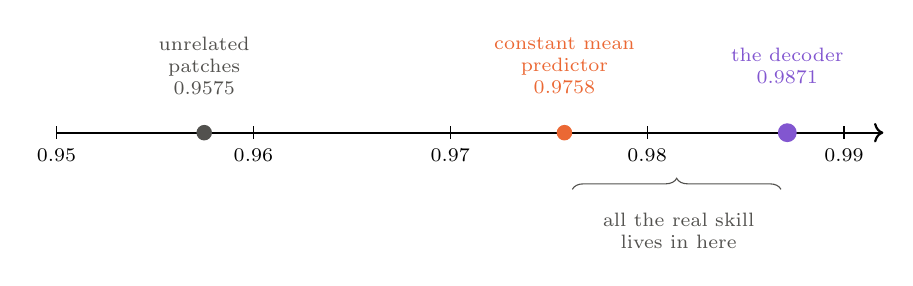
\begin{tikzpicture}[scale=1.0]
\draw[->,thick] (0,0)--(10.5,0);
\foreach \x/\l in {0/0.95,2.5/0.96,5/0.97,7.5/0.98,10/0.99}
  \draw (\x,0.08)--(\x,-0.08) node[below,font=\scriptsize] {\l};
\draw[fill=soft,draw=soft] (1.875,0) circle (2.6pt);
\node[font=\scriptsize,align=center,soft] at (1.875,0.85) {unrelated\\patches\\0.9575};
\draw[fill=warm,draw=warm] (6.45,0) circle (2.6pt);
\node[font=\scriptsize,align=center,warm] at (6.45,0.85) {constant mean\\predictor\\0.9758};
\draw[fill=plum,draw=plum] (9.28,0) circle (3.2pt);
\node[font=\scriptsize,align=center,plum] at (9.28,0.85) {the decoder\\0.9871};
\draw[decorate,decoration={brace,amplitude=4pt},soft] (6.55,-0.72)--(9.2,-0.72);
\node[font=\scriptsize,soft,align=center] at (7.9,-1.25) {all the real skill\\lives in here};
\end{tikzpicture}
\end{center}

The entire achievement of the decoder sits in the gap from $0.9758$ to $0.9871$.
Reporting $0.9871$ without that context would be a serious overstatement.

\begin{codedoes}
The cause is measurable: \textbf{93.1\% of the feature energy lies in the dataset
mean vector.}
\begin{lstlisting}
mu = train_clean.mean(0)
np.linalg.norm(mu)**2 / (test_clean**2).sum(1).mean()   # -> 0.931
\end{lstlisting}
Only 6.9\% of the squared magnitude is the part that distinguishes one patch
from another --- and that part is the only part worth predicting.
\end{codedoes}

\section{The honest metrics}

Two replacements, both measured \emph{relative to the constant-mean baseline}:

\paragraph{Variance explained ($R^2$).}
\[
R^2 \;=\; 1 - \frac{\mathrm{MSE}(\zh, \zc)}{\mathrm{MSE}(\boldsymbol{\mu}, \zc)}
\]
where $\boldsymbol\mu$ is the \emph{training-split} mean. $R^2 = 0$ means no
better than the constant predictor. $R^2 = 1$ means perfect. Negative means
worse than guessing the average.

\paragraph{Centred cosine.} Cosine after subtracting $\boldsymbol\mu$ from both
vectors --- the direction agreement of the part that actually varies.

\begin{flagbox}
$\boldsymbol\mu$ is computed on the \emph{training} split only. Using the test
mean would leak test statistics into the very baseline the decoder is being
scored against.
\end{flagbox}

\section{The control that settles it}

Metrics alone are not enough. The decisive test is the one the main study
already uses for arm C: \textbf{break the correspondence and see what survives}.

\begin{codedoes}
Variant \code{ed\_shuf} is identical to \code{ed} in every respect --- same
architecture, same optimiser, same epochs, same seeds --- except that during
decoder training the radar rows are randomly permuted against their targets. The
decoder therefore sees real radar features, but they belong to the \emph{wrong
patch}. It cannot learn any patch-specific mapping, and its best available
strategy is to output the dataset mean.
\end{codedoes}

\begin{center}
\small
\begin{tabular}{@{}lrrr@{}}
\toprule
& $R^2$ & \textbf{centred cos} & \textbf{raw cos} \\
\midrule
Decoder on real radar     & $+0.4569$ & $0.6403$ & $0.9871$ \\
Decoder on shuffled radar & $-0.0054$ & $0.0540$ & $0.9759$ \\
\midrule
\emph{(constant mean predictor)} & $0.0000$ & $0.0000$ & $0.9758$ \\
\bottomrule
\end{tabular}
\end{center}

\begin{keyfinding}
The shuffled control collapses \emph{exactly} onto the constant-mean predictor:
$R^2 = -0.005$, centred cosine $0.054$, raw cosine $0.9759$ against the mean
predictor's $0.9758$.

\medskip
So the real decoder's $R^2 = 0.457$ is \textbf{genuine, patch-specific learning}.
Radar predicts roughly \textbf{46\% of the patch-to-patch variance} in the clean
optical feature.

\medskip
And note what the raw cosine did: it moved from $0.9759$ to $0.9871$ between a
model that learned \emph{nothing} and a model that learned a real mapping. A gap
of $0.011$. Raw cosine could not have told these two apart.
\end{keyfinding}

%=====================================================================
\chapter{Does the Reconstruction Beat the Damaged Feature?}
\label{ch:recon}

\section{The comparison that matters}

$R^2 = 0.457$ says the decoder beats guessing. But the practical question is
different: at test time you already \emph{have} $\zd$, the damaged optical
feature. Is the radar-derived guess any closer to the truth than what you
already hold?

\begin{center}
\small
\begin{tabular}{@{}rrrrl@{}}
\toprule
\textbf{Masking} & $R^2$ \textbf{of} $\zd$ & $R^2$ \textbf{of} $\zh$ &
\textbf{MSE} $\zh$ / \textbf{MSE} $\zd$ & \textbf{closer to clean?} \\
\midrule
0\%   & $+1.000$ & $+0.457$ & $0.00612 / 0.00000$ & no --- $\zd$ \emph{is} $\zc$ \\
20\%  & $+0.261$ & $+0.457$ & $0.00612 / 0.00833$ & \textbf{yes} \\
40\%  & $-0.530$ & $+0.457$ & $0.00612 / 0.01725$ & \textbf{yes} \\
60\%  & $-1.486$ & $+0.457$ & $0.00612 / 0.02803$ & \textbf{yes} \\
80\%  & $-2.732$ & $+0.457$ & $0.00612 / 0.04209$ & \textbf{yes} \\
100\% & $-6.584$ & $+0.457$ & $0.00612 / 0.08552$ & \textbf{yes} \\
\bottomrule
\end{tabular}
\end{center}

Two things to read off this table.

\paragraph{$\zh$ is flat.} The decoder's accuracy does not depend on the masking
level, because radar is never masked. The row is constant at $0.457$ by
construction. This is the structural advantage of the approach.

\paragraph{$\zd$ goes sharply negative.} Past about 40\% masking, the Vision
Transformer's own output is \emph{further from the clean feature than simply
guessing the dataset average}. At 100\% masking $R^2 = -6.58$: the damaged
feature is actively misleading, not merely uninformative.

\begin{keyfinding}
\textbf{Crossover at $\approx$15\% masking.} Above roughly 15\% cloud, a radar
image predicts the clean optical representation \emph{better than the cloudy
optical image itself does}.

\medskip
Computed by linear interpolation on $R^2_{\zh} - R^2_{\zd}$, which is monotone in
the masking level: the crossing is at $14.7\%$.
\end{keyfinding}

\begin{flagbox}
This is a statement about \emph{feature-space distance}, not about
classification accuracy. Chapter~\ref{ch:cls} shows that classification does not
simply follow --- the two questions have different answers, which is the reason
both are measured.
\end{flagbox}

\begin{center}
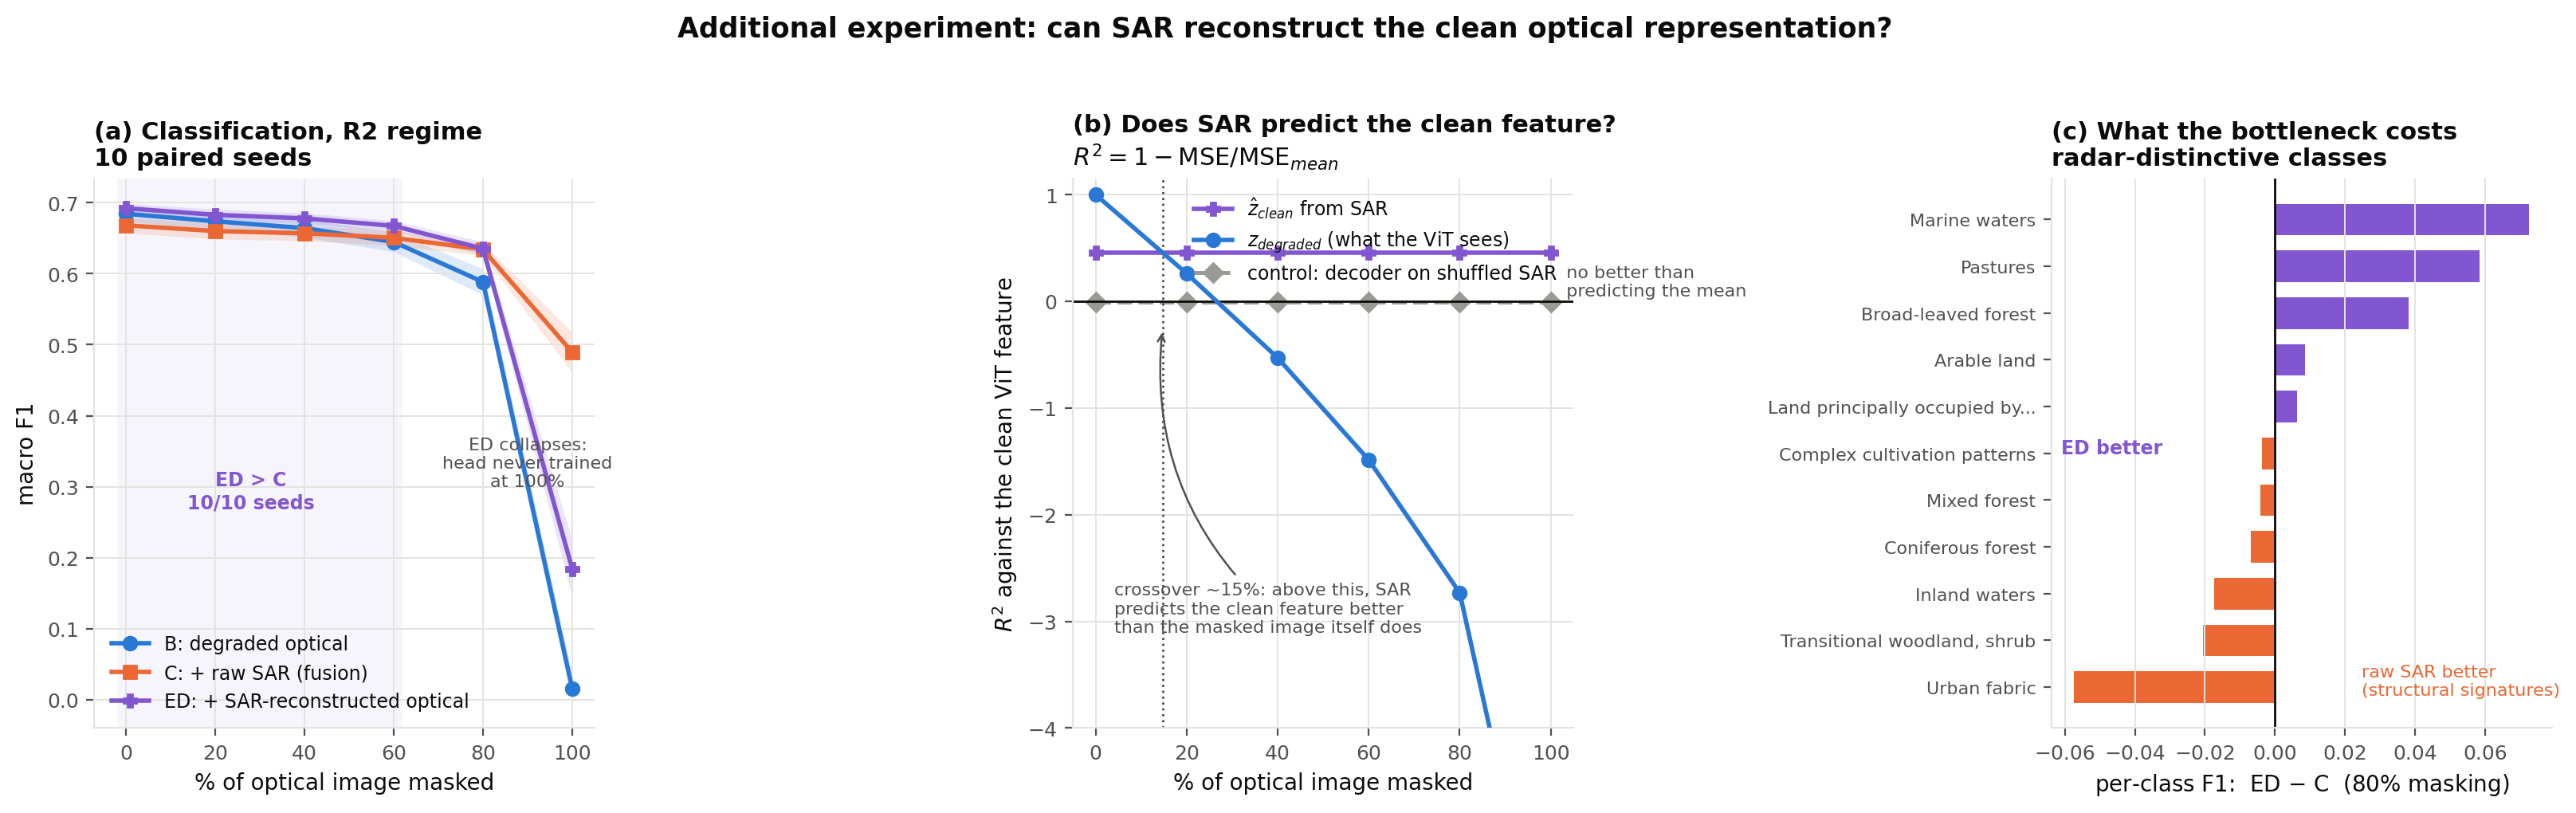
\includegraphics[width=\textwidth]{results/figures/06_encoder_decoder.png}
\end{center}

%=====================================================================
\chapter{Classification Results}
\label{ch:cls}

\section{A methodological detour that changed the headline}

The first run of this experiment, at the project's standard three seeds, put ED
above arm C at 80\% masking by $+0.0074$. Rerunning the identical configuration
gave $-0.0060$.

\begin{flagbox}
\textbf{The sign flipped between two runs of the same code.} MPS (Apple GPU)
kernels are non-deterministic, and the ED-versus-C gap at 80\% is smaller than
the run-to-run spread at three seeds.

\medskip
Had this not been caught, the document would have reported a win that does not
exist. Every ED-versus-C claim was therefore recomputed with \textbf{10 seeds,
with the arms paired seed-for-seed} --- both arms trained in the same process
with the same seed, so the difference is taken within a seed rather than between
independent means.
\end{flagbox}

\section{The matched 10-seed comparison (R2 regime)}

\begin{center}
\small
\begin{tabular}{@{}rrrrrcc@{}}
\toprule
\textbf{Mask} & \textbf{B} & \textbf{C} & \textbf{ED} & \textbf{ED $-$ C} &
\textbf{seeds ED\,$>$\,C} & \textbf{significant} \\
\midrule
0\%   & 0.6843 & 0.6681 & \textbf{0.6921} & $+0.0240$ & 10/10 & yes \\
20\%  & 0.6738 & 0.6600 & \textbf{0.6829} & $+0.0230$ & 10/10 & yes \\
40\%  & 0.6642 & 0.6569 & \textbf{0.6779} & $+0.0210$ & 10/10 & yes \\
60\%  & 0.6447 & 0.6505 & \textbf{0.6673} & $+0.0167$ & 10/10 & yes \\
80\%  & 0.5884 & 0.6341 & 0.6353 & $+0.0012$ & 5/10 & \textbf{no} \\
100\% & 0.0159 & \textbf{0.4894} & 0.1844 & $-0.3051$ & 0/10 & yes \\
\bottomrule
\end{tabular}
\end{center}

``Significant'' here means the mean seed-paired difference exceeds
$1.96 \times$ its standard error over the 10 seeds.

\begin{keyfinding}
Three distinct regimes, and the honest summary needs all three:

\begin{enumerate}
\item \textbf{0--60\% masking: reconstruction wins.} ED beats raw fusion by
      $+0.017$ to $+0.024$, with all 10 seeds agreeing on the sign.
\item \textbf{80\%: a dead heat.} $+0.0012$, 5 seeds out of 10. There is no
      claim to make here.
\item \textbf{100\%: reconstruction fails badly.} $-0.305$, 0 seeds out of 10.
\end{enumerate}
\end{keyfinding}

\section{All arms, both regimes, at three seeds}

For completeness, the full unified table, on the project's standard three seeds
so it lines up exactly with the main study's numbers.

\paragraph{R1 / ED-R1 --- trained on clean optical.}
\begin{center}
\scriptsize
\begin{tabular}{@{}rrrrrr@{}}
\toprule
\textbf{Mask} & \textbf{B optical} & \textbf{C fusion} & \textbf{ED} &
\textbf{shuffled ctrl} & \textbf{D SAR only} \\
\midrule
0\%   & 0.7015 & 0.6916 & \textbf{0.7136} & 0.6773 & 0.6087 \\
20\%  & 0.6181 & \textbf{0.6738} & 0.6644 & 0.5997 & 0.6087 \\
40\%  & 0.5519 & \textbf{0.6438} & 0.6259 & 0.5448 & 0.6087 \\
60\%  & 0.4329 & \textbf{0.6068} & 0.5883 & 0.4781 & 0.6087 \\
80\%  & 0.2835 & \textbf{0.5501} & 0.4870 & 0.2440 & 0.6087 \\
100\% & 0.0093 & \textbf{0.3768} & 0.0802 & 0.0094 & 0.6087 \\
\bottomrule
\end{tabular}
\end{center}

\paragraph{R2 / ED-R2 --- trained with masking augmentation.}
\begin{center}
\scriptsize
\begin{tabular}{@{}rrrrrrr@{}}
\toprule
\textbf{Mask} & \textbf{B optical} & \textbf{C fusion} & \textbf{ED} &
\textbf{ED-residual} & \textbf{shuffled ctrl} & \textbf{D SAR only} \\
\midrule
0\%   & 0.6902 & 0.6771 & 0.6932 & \textbf{0.6983} & 0.6042 & 0.6110 \\
20\%  & 0.6829 & 0.6706 & 0.6860 & \textbf{0.6909} & 0.5862 & 0.6110 \\
40\%  & 0.6734 & 0.6667 & 0.6802 & \textbf{0.6813} & 0.5768 & 0.6110 \\
60\%  & 0.6573 & 0.6595 & \textbf{0.6689} & 0.6650 & 0.5518 & 0.6110 \\
80\%  & 0.6030 & \textbf{0.6403} & 0.6343 & 0.6123 & 0.4957 & 0.6110 \\
100\% & 0.0093 & \textbf{0.4642} & 0.1839 & 0.0093 & 0.0138 & 0.6110 \\
\bottomrule
\end{tabular}
\end{center}

\begin{flagbox}
\textbf{ED-R1 is worse than arm C nearly everywhere} --- at 80\% masking,
$0.4870$ against $0.5501$. This is expected and worth stating plainly: under R1
the head is trained only on clean features, so it never learns to lean on the
reconstruction when the optical half degrades. Reconstruction needs the
degradation-aware regime to pay off.
\end{flagbox}

\begin{center}
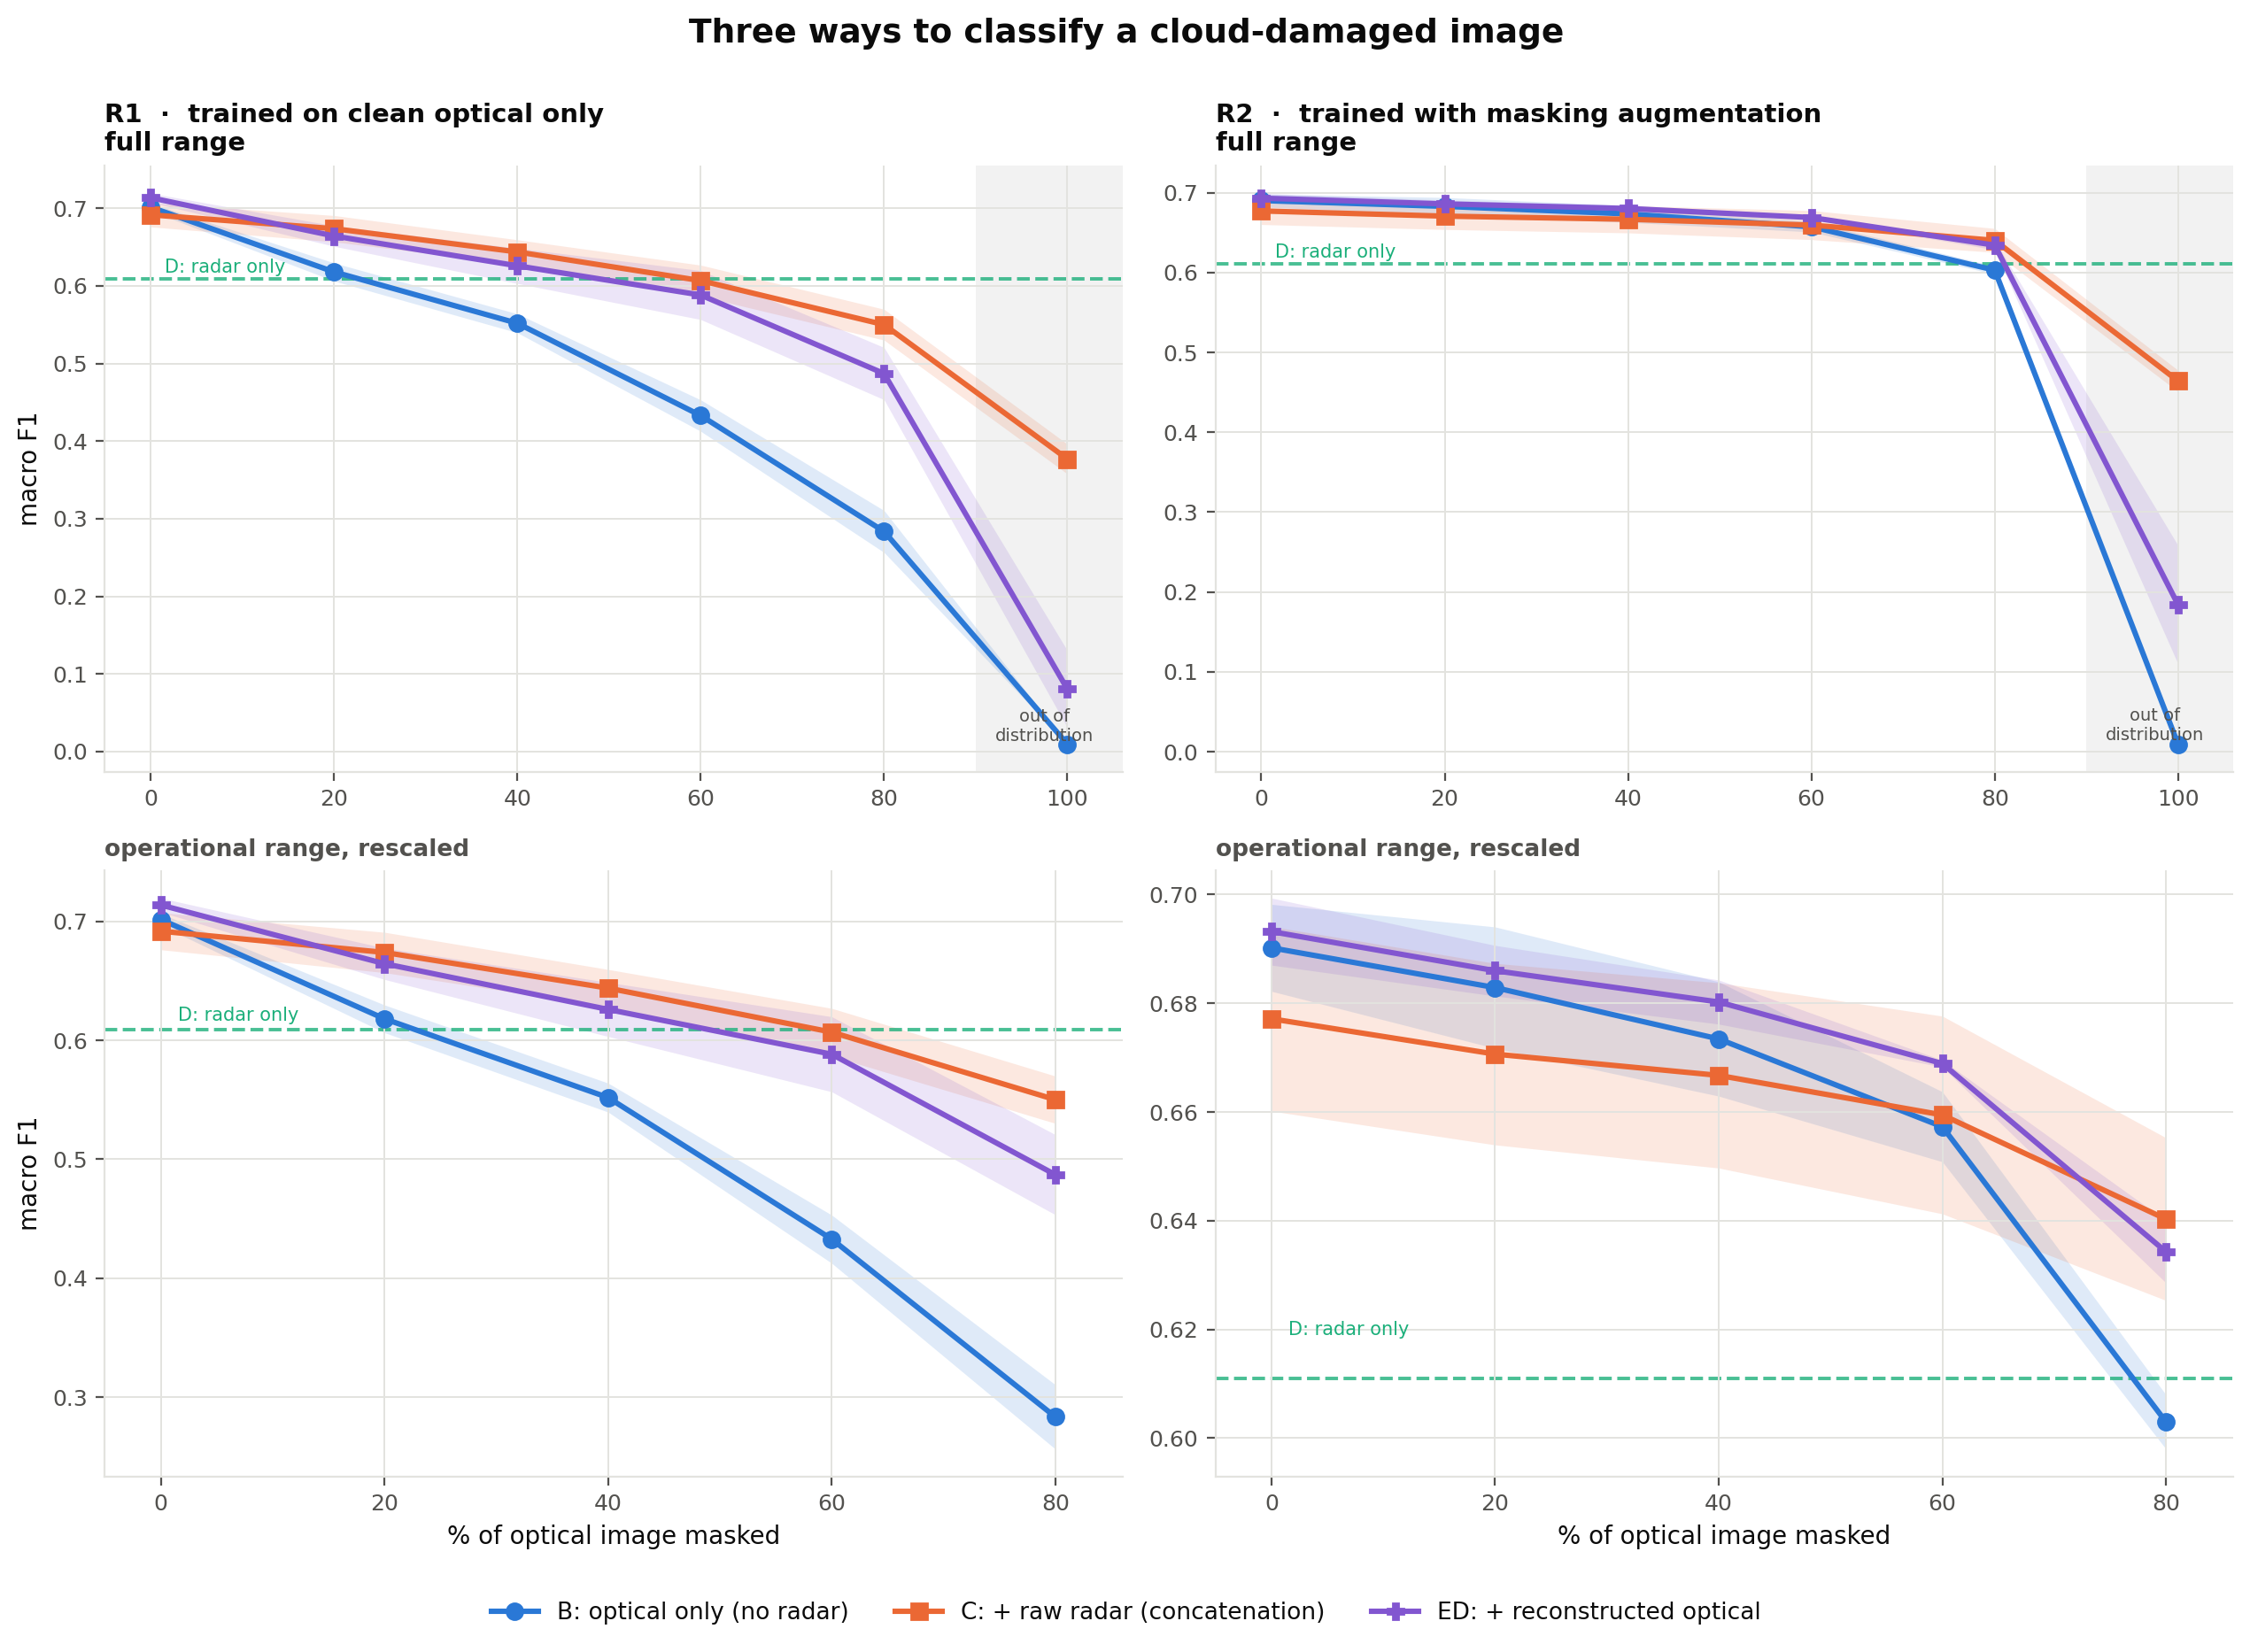
\includegraphics[width=\textwidth]{results/figures/07_three_model_curves.png}
\end{center}

\begin{center}
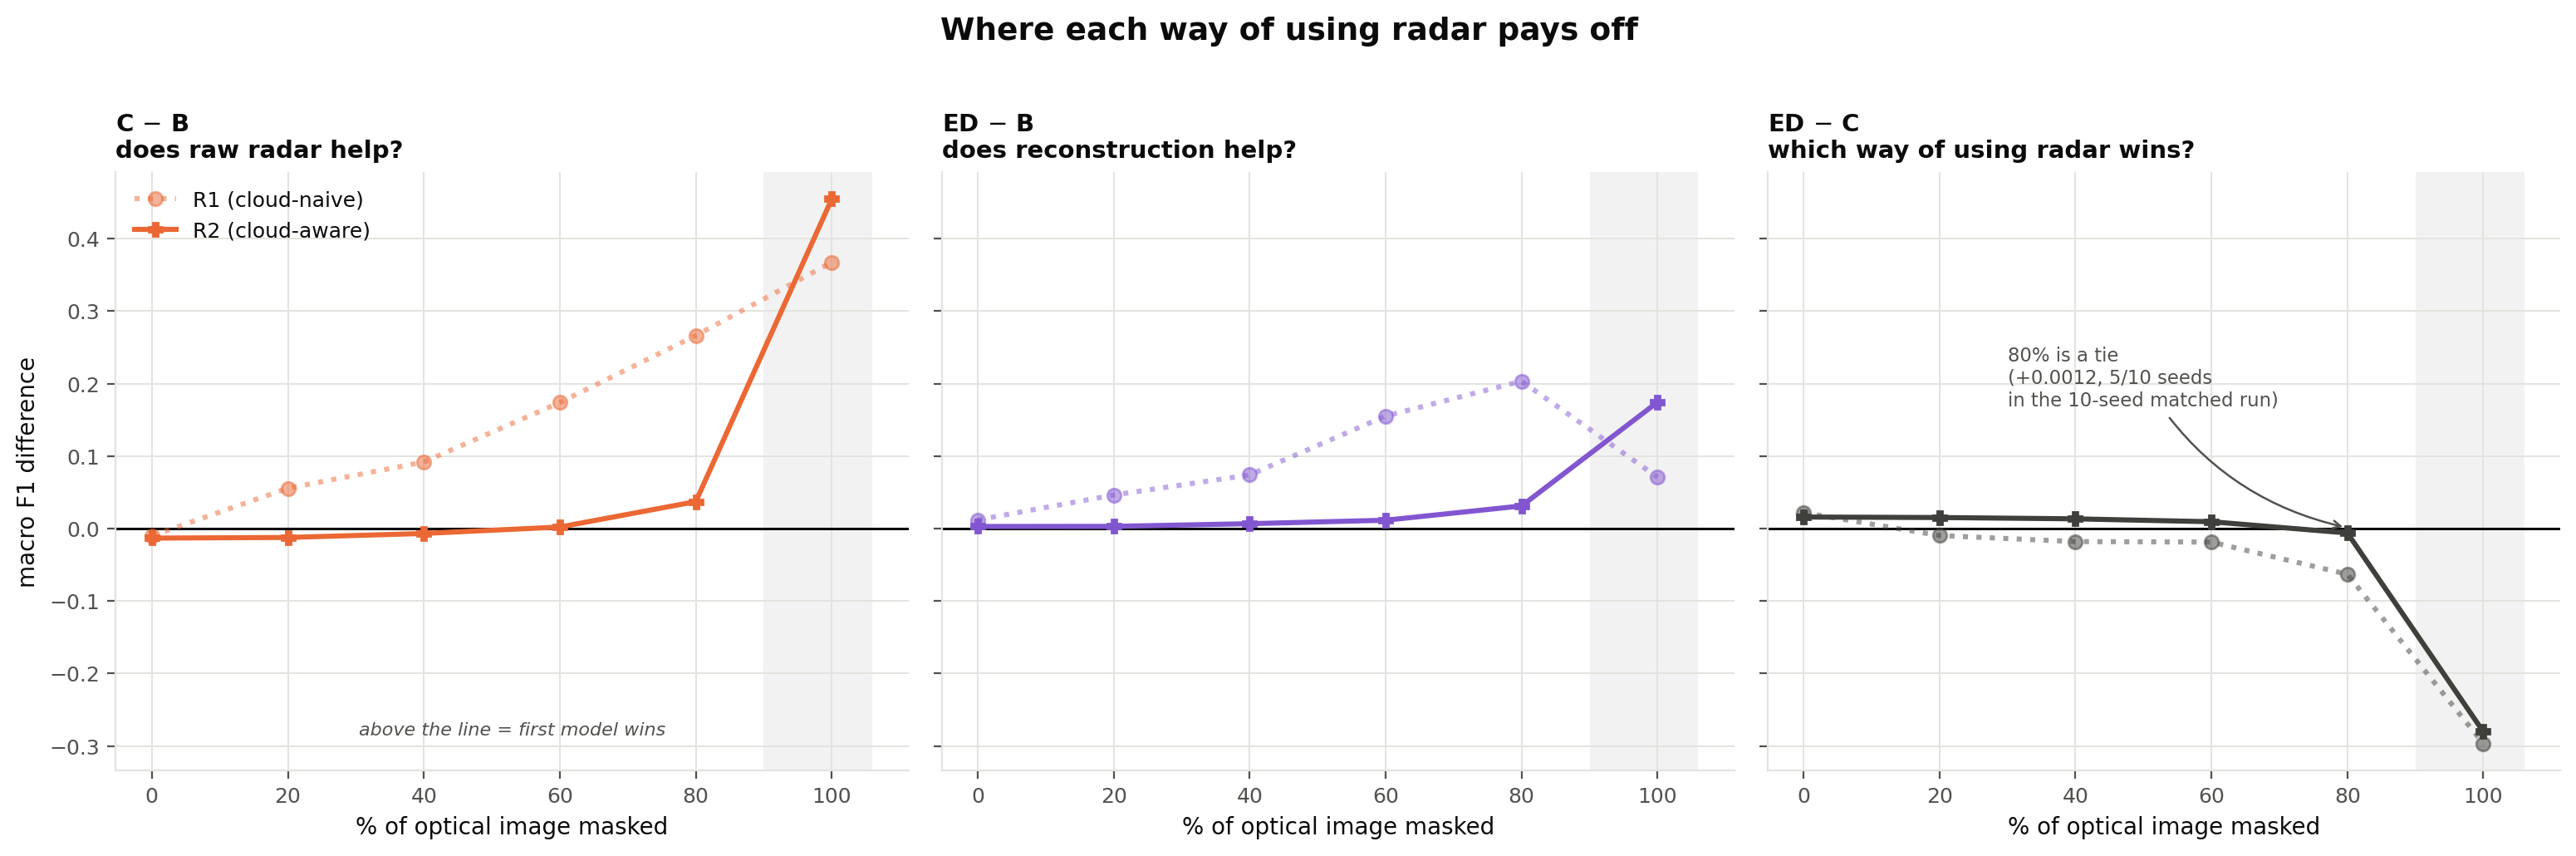
\includegraphics[width=\textwidth]{results/figures/08_three_model_deltas.png}
\end{center}

%=====================================================================
\chapter{Why It Wins Low and Loses High}
\label{ch:why}

\section{Why reconstruction wins at low masking}

Look again at arm C at 0\% masking in the R2 table: $0.6771$, against plain
optical's $0.6902$. \textbf{Adding radar makes things worse when there is no
cloud.}

\begin{intuition}
Arm C hands the classifier 2432 numbers: 384 optical and 2048 radar. The radar
numbers outnumber the optical ones almost 6 to 1, and when the optical image is
undamaged they add nothing --- the answer was already in the 384. The classifier
must learn to ignore most of its input, using 4205 training patches. Some of the
noise gets fitted instead.

\medskip
ED hands it 768 numbers: 384 optical, 384 radar-derived --- and the radar-derived
half is \emph{already expressed in optical coordinates}. Balanced, compact, one
coordinate system.
\end{intuition}

So the reconstruction step acts as a \textbf{learned, task-aligned compression}
of the radar signal: 2048 dimensions down to 384, keeping the part that is
predictive of optical structure. That is why ED is the only arm that never falls
below plain optical in the operational range.

\section{Why it fails at 100\% masking}

At 100\% every pixel is overwritten with the same fill value, so $\zd$ is
identical for every patch --- a constant. The ED input is then
$[\text{constant} \,;\, \zh]$: half of it is dead weight.

Arm C survives better because its 2048 raw radar dimensions dominate the input,
so the constant optical block matters proportionally less.

\begin{flagbox}
\textbf{This is a flaw in the experimental design, not a property of
reconstruction.} The R2 training levels are
$\{0, 0.2, 0.4, 0.6, 0.8\}$ --- \textbf{1.0 is not among them}. The head has
never seen a fully blank optical input and is out of distribution when it meets
one.

\medskip
Adding $1.0$ to \code{train\_levels} would very likely fix it. The same flaw
affects arm C in the main study and is documented there. The 100\% column should
be read as a bound, not an operating point.
\end{flagbox}

%=====================================================================
\chapter{Per-Class Effects: What the Bottleneck Costs}
\label{ch:perclass}

\section{The trade, class by class}

At 80\% masking, R2 regime, ED minus C per class:

\begin{center}
\small
\begin{tabular}{@{}lrrp{6.6cm}@{}}
\toprule
\textbf{Class} & \textbf{support} & \textbf{ED $-$ C} & \textbf{Reading} \\
\midrule
Marine waters        & 116  & $+0.073$ & but see the confound below \\
Pastures             & 916  & $+0.058$ & spectrally distinctive \\
Broad-leaved forest  & 511  & $+0.038$ & \\
Arable land          & 883  & $+0.008$ & \\
Land principally agri.\ & 996 & $+0.006$ & \\
Complex cultivation  & 1172 & $-0.004$ & \\
Mixed forest         & 1214 & $-0.004$ & \\
Coniferous forest    & 1193 & $-0.007$ & \\
Inland waters        & 379  & $-0.017$ & specular return is radar-specific \\
Transitional woodland & 885 & $-0.020$ & structural, not spectral \\
Urban fabric         & 265  & $-0.057$ & double-bounce is radar-specific \\
\bottomrule
\end{tabular}
\end{center}

\begin{keyfinding}
The classes where \textbf{raw fusion still beats reconstruction} are exactly
those with \textbf{distinctive radar signatures that have no optical
analogue}:

\begin{itemize}
\item \textbf{Urban fabric.} Buildings meeting the ground form a corner
      reflector, sending the radar pulse straight back --- a
      \emph{double-bounce} signature. Bright and unmistakable in radar, and not
      a colour fact at all.
\item \textbf{Inland waters.} Calm water is a mirror at radar wavelengths;
      the pulse reflects away and almost nothing returns, so water is nearly
      black. Again, a geometry fact, not a colour fact.
\end{itemize}

Forcing radar through a ``predict the optical feature'' bottleneck
\textbf{necessarily discards these}, because there is no optical feature for
them to map onto. That is the conceptual cost of the reconstruction framing, and
it shows up in the per-class numbers rather than needing to be argued.
\end{keyfinding}

\begin{flagbox}
\textbf{Do not lean on the Marine waters number.} It is the largest ED gain in
the table, and it is also the least trustworthy: all 116 Marine-waters test
patches are exactly the 116 test patches from the second tile, T34UDG. So
``reconstruction helps Marine waters'' is entangled with ``reconstruction
behaves differently on the tile that contributes almost no other test data''.
This confound is documented in the main study's limitations and applies
unchanged here.
\end{flagbox}

\begin{center}
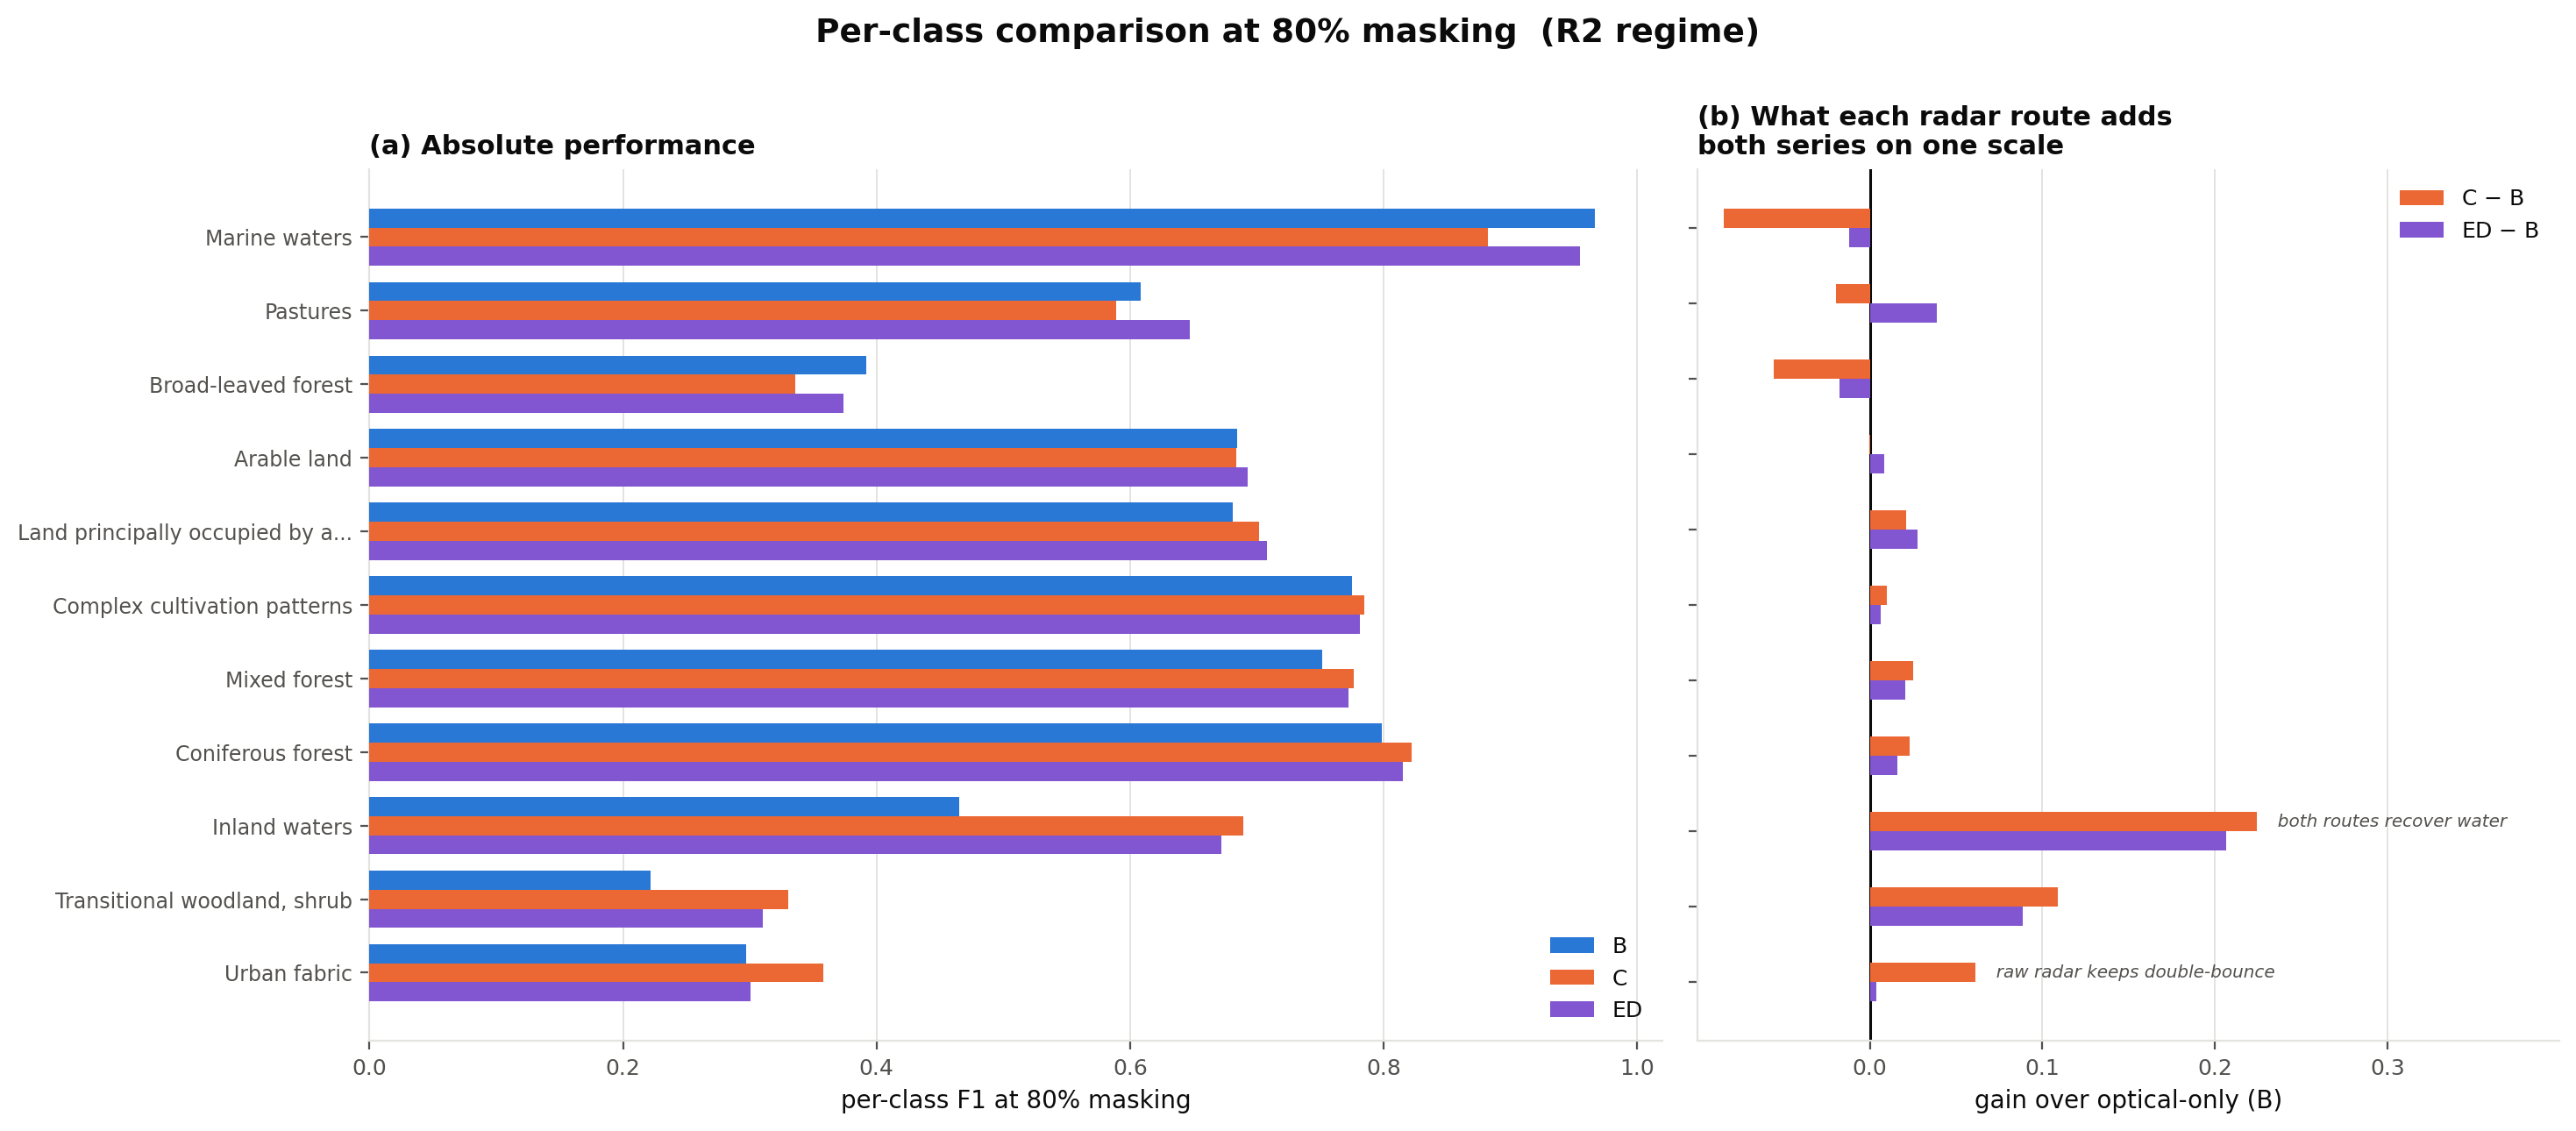
\includegraphics[width=\textwidth]{results/figures/09_three_model_per_class.png}
\end{center}

\section{Error structure}

\begin{center}
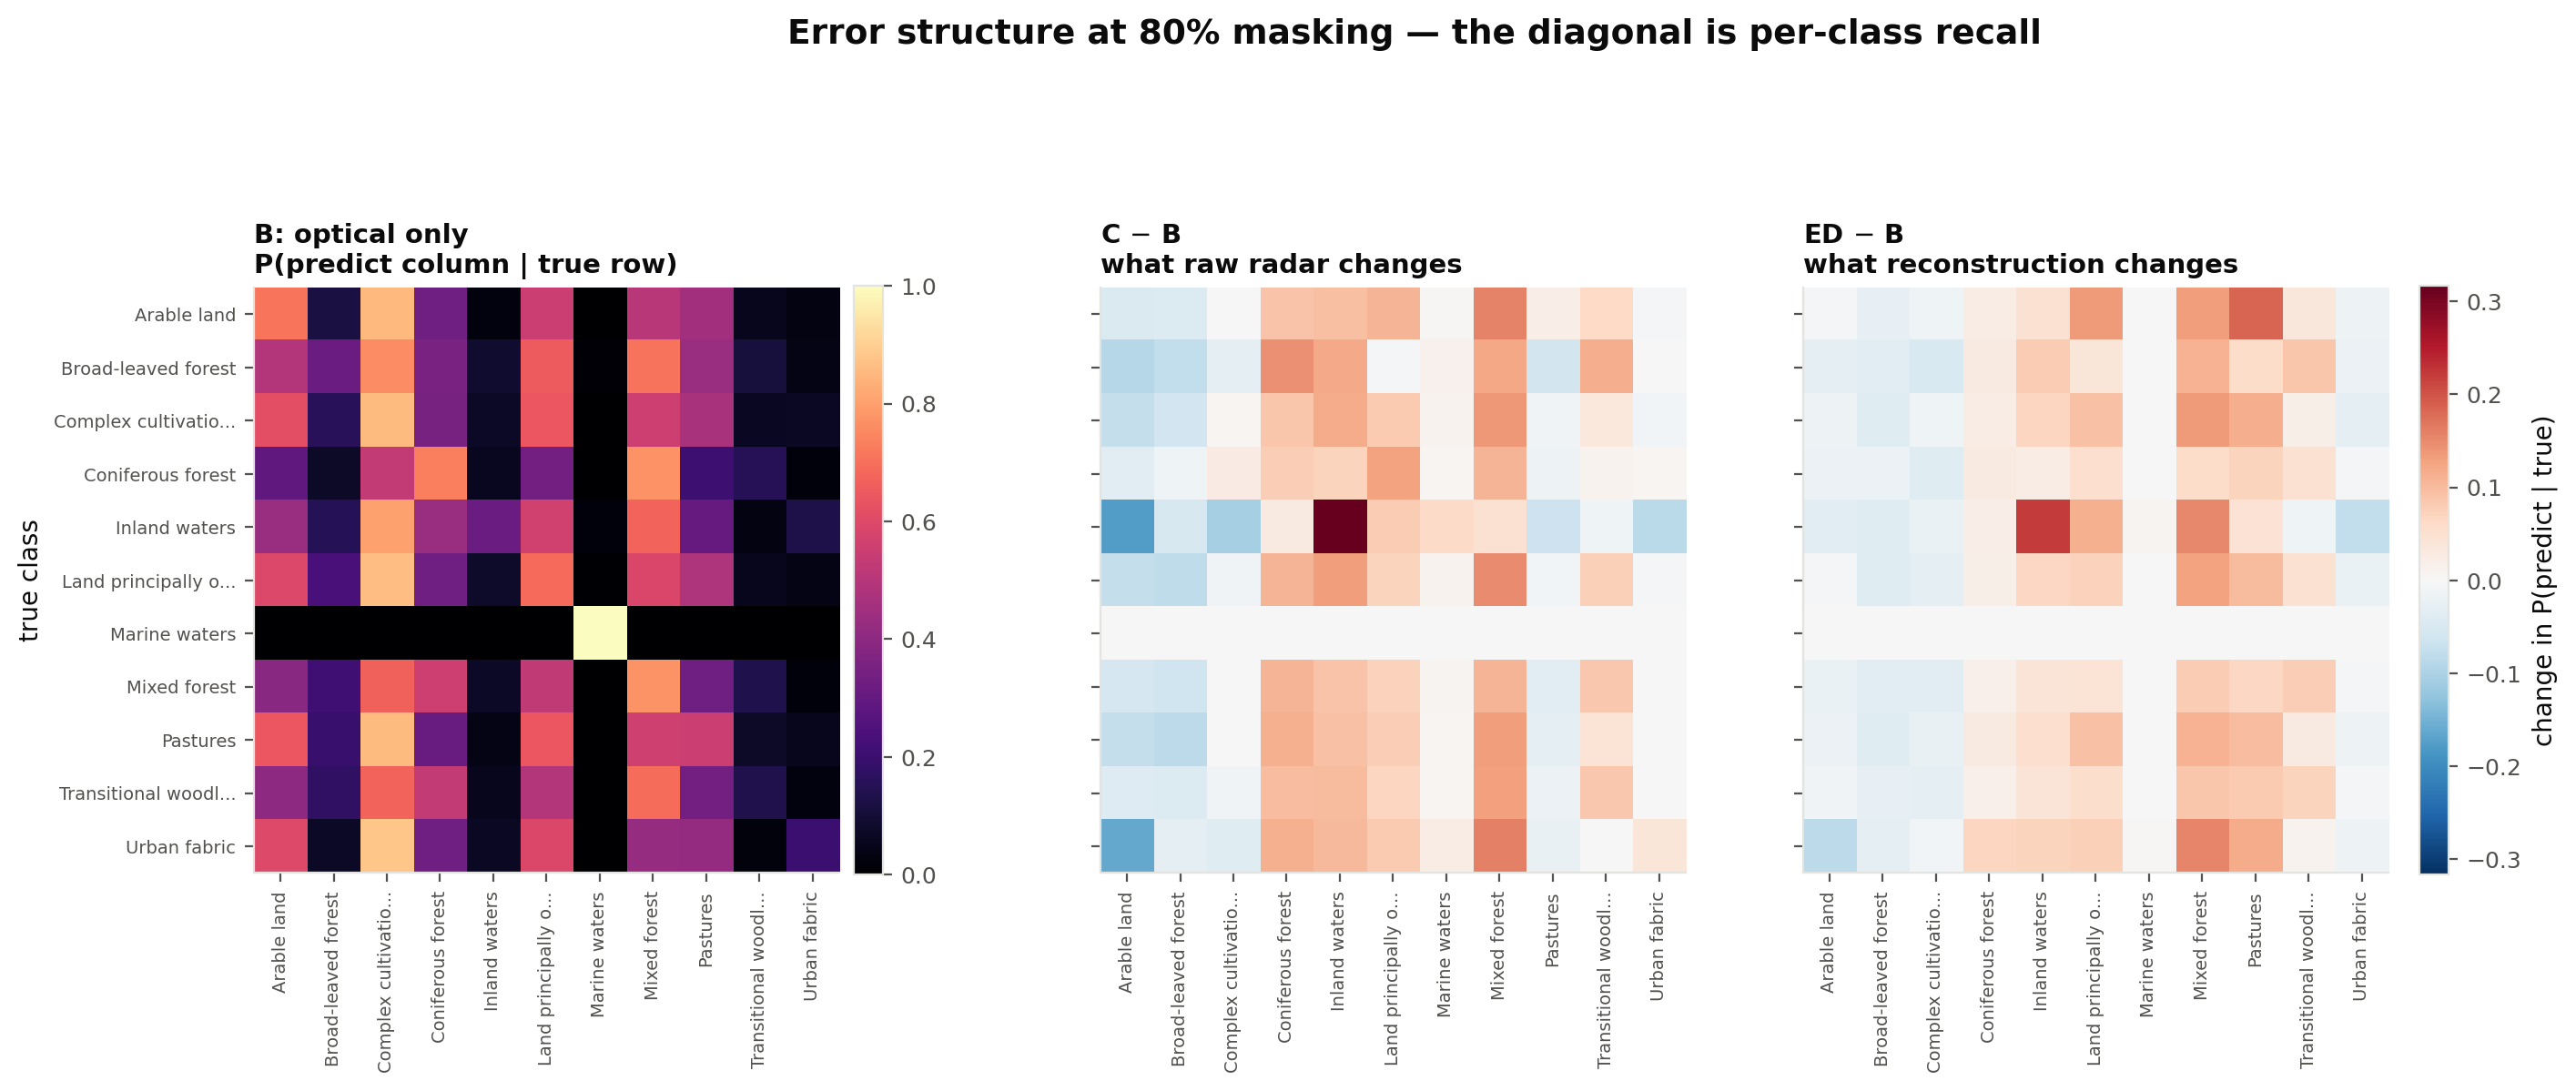
\includegraphics[width=\textwidth]{results/figures/10_three_model_error_matrices.png}
\end{center}

Entry $(i,j)$ is $P(\text{predict } j \mid \text{patch truly contains } i)$. The
diagonal is per-class recall; off-diagonal mass shows which classes get dragged
along. Comparing the three panels shows \emph{which confusions} each way of
using radar resolves, rather than only how many.

%=====================================================================
\chapter{Patch-Level Behaviour}
\label{ch:qual}

\section{The aggregate hides enormous disagreement}

At 80\% masking the two arms differ by $+0.0012$ macro F1 --- effectively a tie.
It would be easy to conclude they behave the same way. They do not.

\begin{center}
\small
\begin{tabular}{@{}lrr@{}}
\toprule
\textbf{At 80\% masking, over 2151 test patches} & \textbf{count} & \textbf{share} \\
\midrule
ED strictly better than C (by $>0.05$ per-patch F1) & 568 & 26.4\% \\
C strictly better than ED (by $>0.05$)              & 553 & 25.7\% \\
Tied within 0.05                                    & 1030 & 47.9\% \\
\bottomrule
\end{tabular}
\end{center}

\begin{keyfinding}
The two approaches disagree on \textbf{more than half of all patches}, in
almost perfectly balanced directions. The tie in the aggregate is not agreement
--- it is two large opposing effects cancelling.

\medskip
That is a much more interesting result than ``no difference'', and it is the
strongest argument for the routing idea in Chapter~\ref{ch:next}: if you could
tell in advance which patches belong in which group, you would beat both arms.
\end{keyfinding}

\section{Representative cases}

Selection rules are fixed in the code before any result is inspected, and
\textbf{two of the four categories are cases where reconstruction is the worse
choice}, included by construction.

\begin{center}
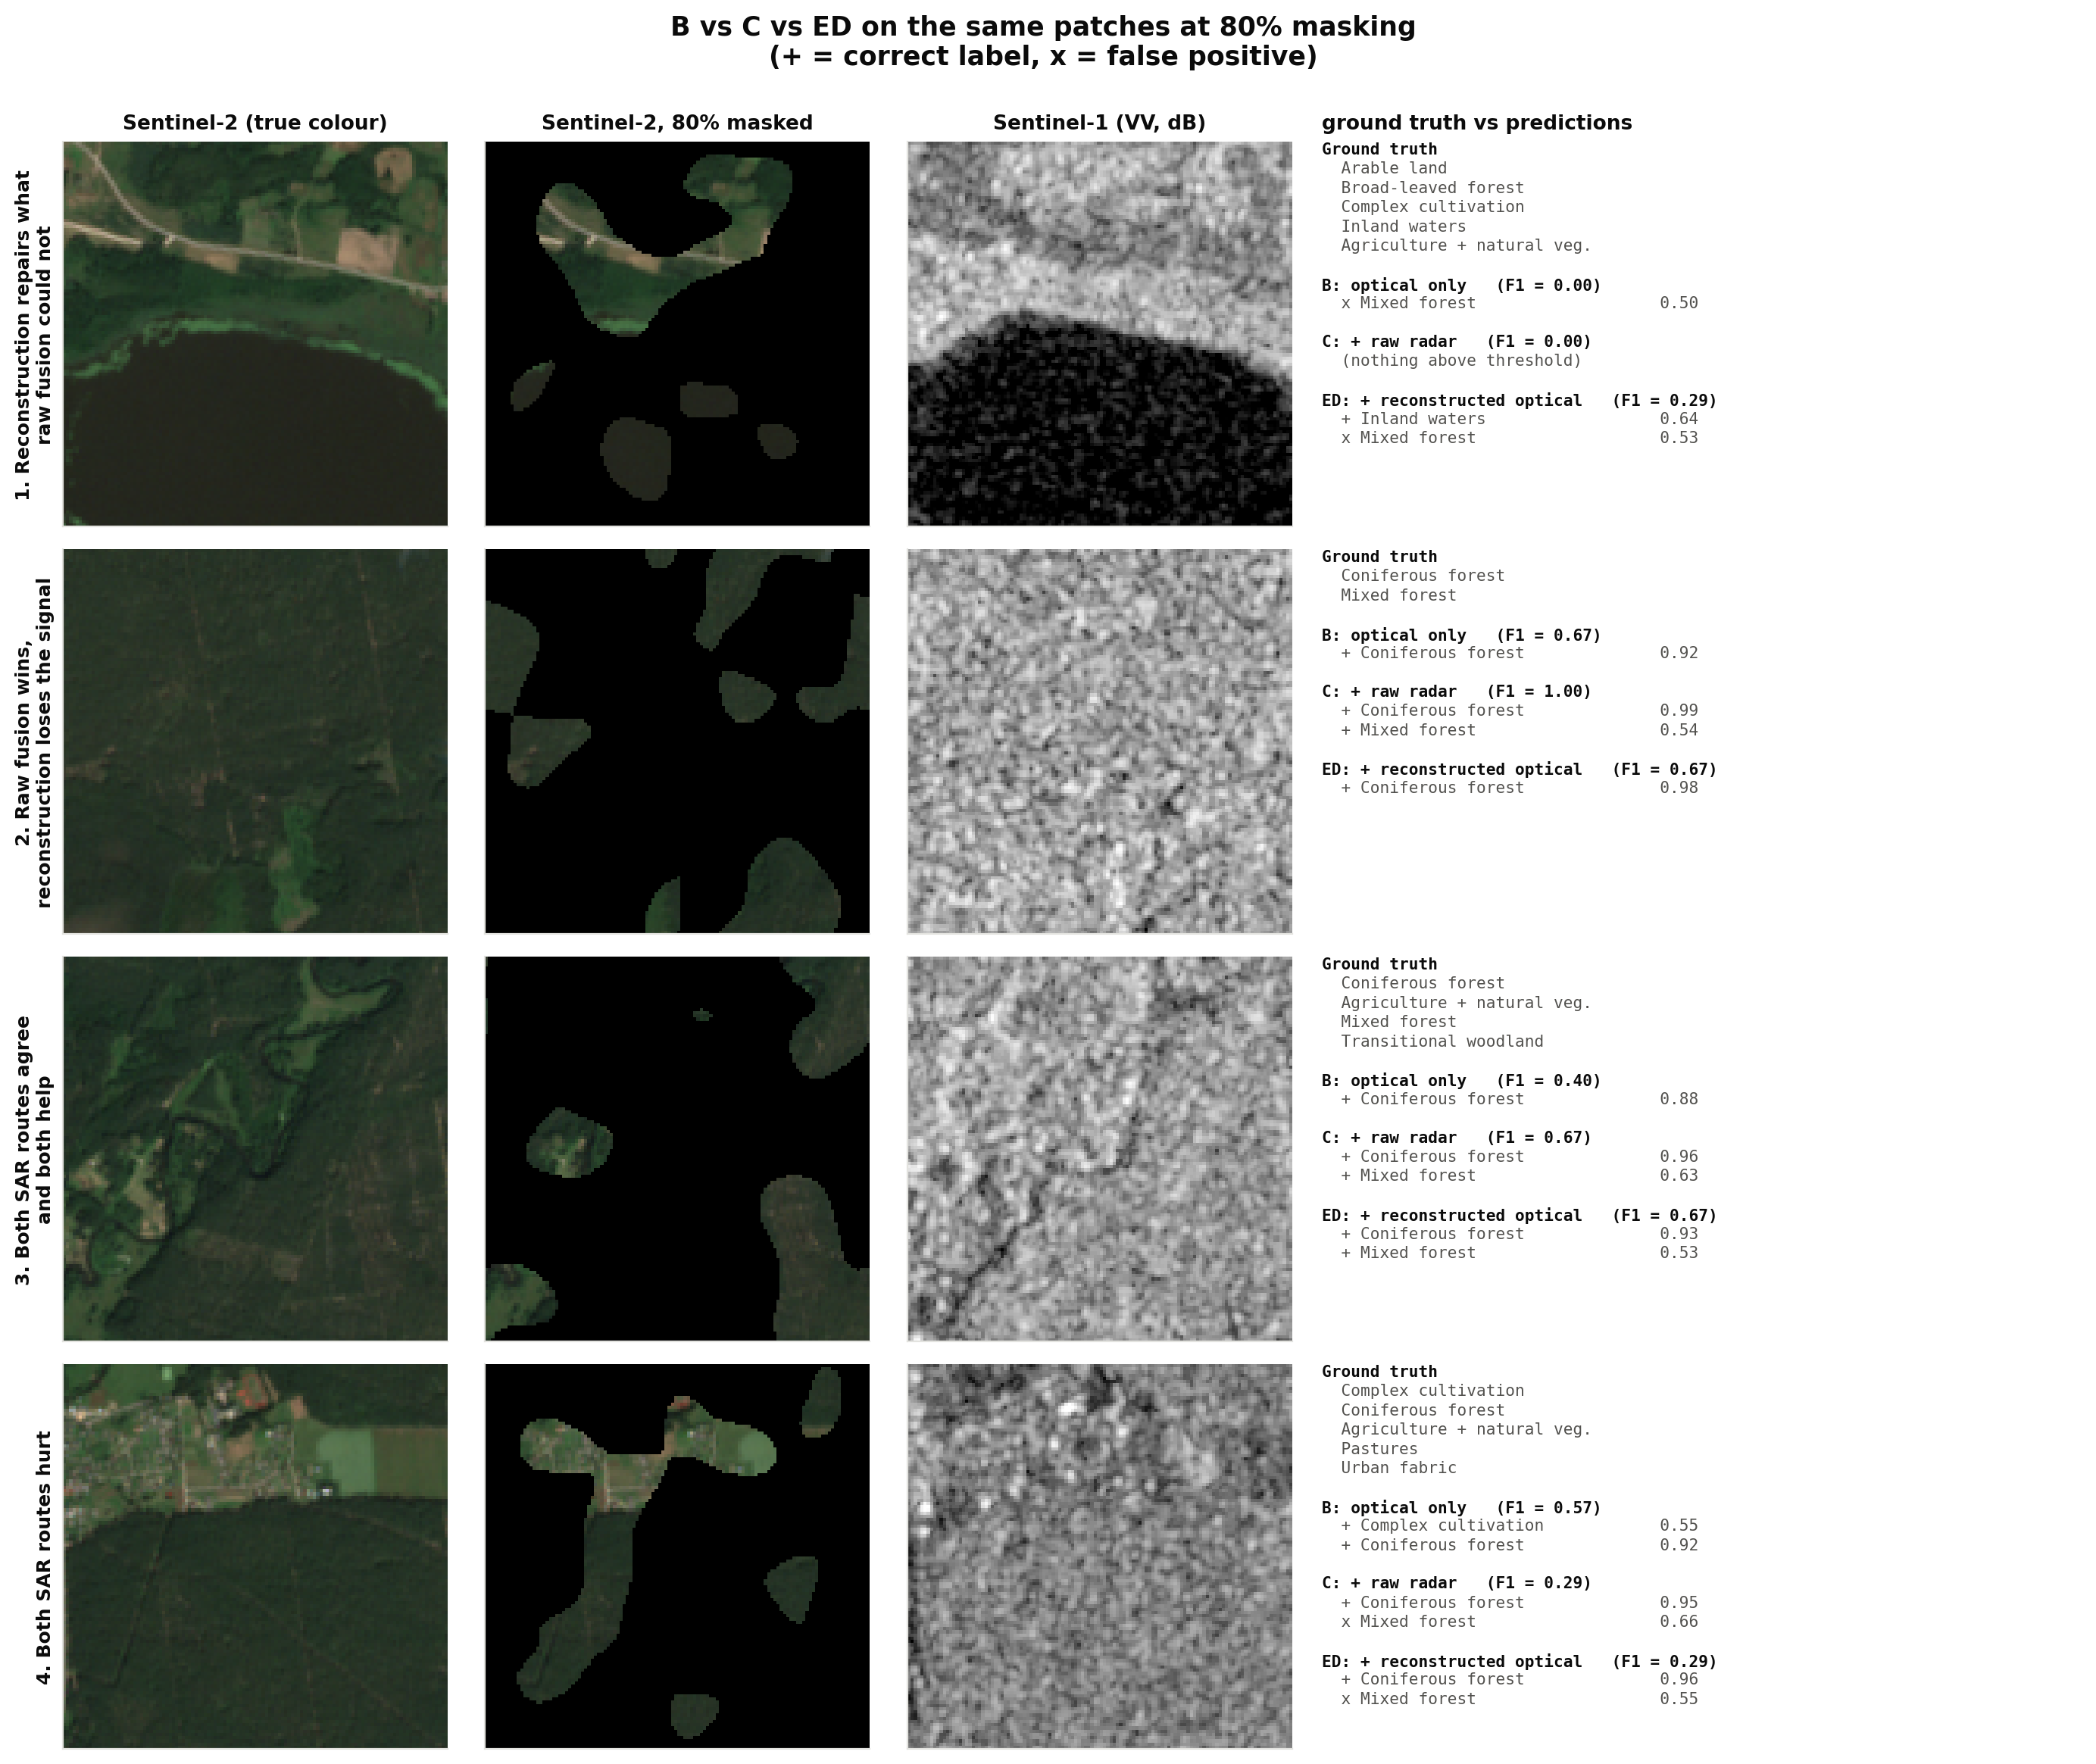
\includegraphics[width=\textwidth]{results/figures/11_three_model_qualitative_L080.png}
\end{center}

\paragraph{Row 1 --- reconstruction repairs what fusion could not.} A lakeside
patch. The radar panel shows a large black region: calm water, mirror-like,
almost no return. Arm B predicts one wrong label; arm C predicts
\emph{nothing at all} above threshold. ED recovers \emph{Inland waters} at
confidence 0.64. The radar evidence was equally available to arm C --- putting
it through the optical bottleneck is what made it usable.

\paragraph{Row 2 --- fusion wins, reconstruction loses the signal.} Conifer and
mixed forest. Arm C gets both labels (F1 = 1.00); ED gets only coniferous
(F1 = 0.67). The structural distinction between canopy types is exactly the kind
of information that does not survive projection into optical feature space.

\paragraph{Rows 3 and 4.} Both routes agree and help; both routes hurt. Radar
adds a false \emph{Mixed forest} label in row 4 regardless of how it is used ---
a failure of the radar signal itself, not of either architecture.

%=====================================================================
\chapter{The Residual Variant}
\label{ch:res}

\section{The idea}

Rather than predicting the clean feature outright, predict the \emph{missing
part}:
\[
\boldsymbol\Delta = \zc - \zd, \qquad
\zh = \zd + \hat{\boldsymbol\Delta}
\]
Intuitively appealing: the decoder only has to supply what cloud destroyed, not
re-derive what is still visible.

\section{Why it is limited by construction}

\begin{flagbox}
The decoder sees \emph{only} radar. Radar does not change with the masking
level. But $\boldsymbol\Delta$ \emph{does} --- the residual at 20\% masking is
much smaller than at 80\%.

\medskip
So the decoder is being asked to predict a quantity that depends on information
it is not given. Under MSE its best strategy is to predict the \emph{average}
residual across the training levels. It cannot condition on how cloudy the image
actually is.
\end{flagbox}

This is visible directly in the numbers: it reconstructs \emph{better} than the
direct variant at low masking and much worse at high masking.

\begin{center}
\small
\begin{tabular}{@{}rrr@{}}
\toprule
\textbf{Masking} & $R^2$ \textbf{direct} & $R^2$ \textbf{residual} \\
\midrule
0\%   & $+0.457$ & $+0.182$ \\
20\%  & $+0.457$ & $\mathbf{+0.605}$ \\
40\%  & $+0.457$ & $+0.521$ \\
60\%  & $+0.457$ & $+0.167$ \\
80\%  & $+0.457$ & $-0.593$ \\
100\% & $+0.457$ & $-6.292$ \\
\bottomrule
\end{tabular}
\end{center}

Classification tracks this exactly: marginally better than direct at 0--40\%,
clearly worse at 80\% ($0.6123$ vs $0.6343$), and fully degenerate at 100\%
($0.0093$ --- the single-class collapse).

It is also R2-only: under R1 the residual target is identically zero, so the
variant is meaningless there and the run is skipped rather than reported.

\begin{whybox}
Reported for completeness because it was worth testing, but \textbf{the direct
variant is the better formulation}. The obvious fix --- give the decoder the
estimated cloud fraction, or $\zd$ itself, as an additional input --- is listed
in Chapter~\ref{ch:next}.
\end{whybox}

%=====================================================================
\chapter{Leakage: Proving the Answer Key Was Not Peeked At}
\label{ch:leak}

The experiment is worthless if $\zc$ leaks into inference. The clean feature is
the regression target; if it were also available at test time, the whole thing
would be circular.

Reasoning about the code is not sufficient evidence, so this is verified
empirically on trained models by \file{scripts/11\_ed\_leakage\_audit.py}.

\section{The five checks}

\paragraph{1. Destroy the answer key and see if anything changes.}
The strongest test available. Overwrite every clean test feature with random
noise, then re-run inference:

\begin{center}
\small
\begin{tabular}{@{}lr@{}}
\toprule
\textbf{Perturbation} & \textbf{Change in ED test predictions} \\
\midrule
Overwrite $\zc$ (the target) with noise & $\max|\Delta| = 0.00\mathrm{e}{+}00$ \\
Overwrite $\zd$ (the real input) with noise & mean $|\Delta| = 0.174$ \\
\bottomrule
\end{tabular}
\end{center}

The predictions are \textbf{bit-identical} when the clean feature is destroyed.
And the second row matters just as much: destroying the feature that
\emph{is} used does change the output, so the first test is not passing
vacuously.

\paragraph{2. Decoder output ignores optical entirely.} Calling the decoder with
the clean optical feature alongside, versus the 100\%-masked one, gives
identical output.

\paragraph{3. The decoder physically rejects optical input.} Its
\code{forward()} raises \code{ValueError} on any tensor of width 384. A clean
feature cannot be fed in even by mistake.

\paragraph{4. The decoder never saw a label.} It maps $2048 \rightarrow 384$;
neither dimension is the 11-class label space, and \code{train\_decoder()} takes
no label tensor.

\paragraph{5. Targets never came from a test patch.} Train (4205), validation
(2418) and test (2151) patch ids are pairwise disjoint.

\begin{codedoes}
All five run in one command:
\begin{lstlisting}
python scripts/11_ed_leakage_audit.py
\end{lstlisting}
Every check is an assertion --- the script fails loudly rather than printing a
warning.
\end{codedoes}

%=====================================================================
\chapter{Limitations}
\label{ch:lim}

Stated plainly, worst first.

\paragraph{Everything is frozen.} The decoder can only work with what SSL4EO's
ResNet-50 already encodes. A fine-tuned radar encoder might carry considerably
more optically-predictive signal. $R^2 = 0.457$ is a statement about \emph{this
frozen encoder}, not about radar in general.

\paragraph{Two-stage, not joint.} Deliberate (Chapter~\ref{ch:train}), but it
means ED is not the best achievable version of this idea.

\paragraph{The reconstruction is level-invariant.} $\zh$ does not know how much
of the image is missing. A decoder conditioned on estimated cloud fraction
should do better, and the residual variant's failure is direct evidence for
this.

\paragraph{$R^2 = 0.457$ is a mid-range number.} Radar explains under half the
patch-to-patch variance. The reconstruction is real but partial, and
Chapter~\ref{ch:perclass} shows it is systematically biased toward what is
spectrally rather than structurally distinctive.

\paragraph{The 100\% column is an artefact.} Out of distribution for a head
trained only to 80\%. It bounds behaviour; it does not describe it.

\paragraph{Three seeds is too few, ten is better but not many.} The 80\%
ED-versus-C comparison is genuinely unresolved.

\paragraph{Everything inherited from the main study still applies.} Two
Sentinel-2 tiles, two acquisition dates, one country, one season. Synthetic
cloud masks with hard edges and no shadow. The Marine-waters/tile confound.
Non-simultaneous Sentinel-1/Sentinel-2 pairing. The effective sample size for
any geographic generalisation claim is closer to two satellite passes than to
8{,}774 images.

\paragraph{The physical explanations are interpretation.} Double-bounce and
specular reflection are standard radar physics and they fit the per-class
pattern, but no ablation of scattering mechanisms was run. Read
Chapter~\ref{ch:perclass}'s mechanism claims as ``consistent with'', not
``demonstrated''.

%=====================================================================
\chapter{What I Would Do Next}
\label{ch:next}

In order of expected value.

\begin{enumerate}
\item \textbf{Route between the two arms on estimated cloud fraction.}
      Chapter~\ref{ch:qual} shows the arms disagree on 52\% of patches in
      near-perfectly balanced directions. A selector using reconstruction below
      $\sim$60\% masking and raw fusion above it should beat both, and the
      crossover is already measured.
\item \textbf{Condition the decoder on cloud fraction.} Feed the estimated
      masking level, or $\zd$ itself, as an extra decoder input. This directly
      fixes the residual variant's failure mode and makes $\zh$ adaptive rather
      than flat.
\item \textbf{Add 1.0 to \code{train\_levels}.} Removes the 100\% artefact for
      both ED and arm C. Costs one line and about a minute.
\item \textbf{Blend rather than concatenate.} Feed
      $\alpha\,\zd + (1-\alpha)\,\zh$ with $\alpha$ falling as cloud rises,
      instead of concatenating both. Keeps the input at 384 and makes the
      substitution explicit.
\item \textbf{Train the decoder jointly with the head}, and report it
      \emph{alongside} the two-stage version rather than instead of it --- the
      two-stage reconstruction metric is what makes the claim falsifiable.
\item \textbf{More tiles and more seasons.} As in the main study, this dominates
      every architectural improvement.
\item \textbf{Unfreeze the radar encoder} --- only after the above, since it
      reintroduces the capacity confound the frozen design exists to exclude.
\end{enumerate}

%=====================================================================
\chapter{How to Explain This in an Interview}

\section{The thirty-second version}

\begin{quote}
``The fusion arm asks whether radar is useful alongside cloudy optical. I added a
second arm asking something stronger --- whether radar can \emph{predict} the
optical representation a clean image would have produced. It can: $R^2$ of 0.46
against a shuffled-radar control at zero. And it turns out to classify better
than plain concatenation below 60\% cloud, because it compresses 2048 radar
dimensions into 384 already aligned with the optical space instead of making the
classifier sort that out. Above 60\% it loses, because the bottleneck discards
exactly the radar-only signals --- urban double-bounce, specular water.''
\end{quote}

\section{The story worth telling}

Not the result --- the control.

\begin{quote}
``My first reconstruction score was a cosine similarity of 0.987, which looks
like a solved problem. Before reporting it I checked what a model that learned
nothing would score. A constant predictor that always outputs the dataset mean
gets 0.976, and two completely unrelated patches sit at 0.958 --- 93\% of the
feature energy is in the mean vector. So my apparently excellent number was
0.011 above cheating.

\smallskip
I switched to variance explained relative to that baseline and added a
shuffled-radar control, the same control the main study uses for fusion. The
control landed at $R^2 = -0.005$, exactly the mean predictor, which is what
confirmed the real decoder's 0.46 was genuine patch-specific learning. The
finding survived; the metric I would have reported it with did not.''
\end{quote}

\section{Questions to expect}

\begin{center}
\small
\begin{tabular}{@{}p{5.4cm}p{9.4cm}@{}}
\toprule
\textbf{Question} & \textbf{Answer} \\
\midrule
``Is 0.46 good?'' &
``Mid-range, and I would not oversell it. Radar explains under half the
patch-to-patch variance. What makes it credible is the control at $-0.005$, not
the magnitude.'' \\
\addlinespace
``Why not train it end to end?'' &
``It would score better and I would learn less. A jointly-trained decoder is a
reparameterised fusion head, and the reconstruction metric stops being
independent evidence.'' \\
\addlinespace
``You beat fusion at 80\%, right?'' &
``No. My first 3-seed run said $+0.007$; the rerun said $-0.006$. At 10 paired
seeds it is $+0.001$ with 5 seeds out of 10 --- a tie. I only claim the win
below 60\%.'' \\
\addlinespace
``Why does it fail at 100\%?'' &
``My design flaw, not a property of reconstruction. R2 trains up to 80\%, so the
head has never seen a constant optical input. Should have included 1.0.'' \\
\addlinespace
``So which approach is better?'' &
``Neither dominates, and I think that is the actual finding. They disagree on
52\% of patches in balanced directions. The useful next step is routing between
them, not picking one.'' \\
\bottomrule
\end{tabular}
\end{center}

%=====================================================================
\chapter{Verification Log}
\label{ch:verify}

Every non-obvious number in this document, with its source.

\begin{center}
\scriptsize
\begin{longtable}{@{}p{6.9cm}rp{5.6cm}@{}}
\toprule
\textbf{Claim} & \textbf{Value} & \textbf{Source} \\
\midrule
\endhead
Decoder $R^2$ against clean feature & $+0.4569$ & \file{ed\_reconstruction.csv}, \code{r2\_hat} \\
Decoder centred cosine & $0.6403$ & \file{ed\_reconstruction.csv} \\
Decoder raw cosine & $0.9871$ & \file{ed\_reconstruction.csv} \\
Shuffled-radar control $R^2$ & $-0.0054$ & \file{ed\_reconstruction.csv}, \code{variant=ed\_shuf} \\
Shuffled-radar centred cosine & $0.0540$ & same \\
Constant mean predictor, cosine & $0.9758$ & computed from \file{train\_opt\_L000.npy} \\
Two unrelated patches, cosine & $0.9575$ & computed from \file{test\_opt\_L000.npy} \\
Feature energy in the mean vector & $93.1\%$ & $\|\mu\|^2 / \mathbb{E}\|z\|^2$ \\
$R^2$ of degraded feature, 0--100\% & $1.000$ to $-6.584$ & \file{ed\_reconstruction.csv}, \code{r2\_degraded} \\
Reconstruction/degradation crossover & $14.7\%$ & interpolation, \file{10\_ed\_figures.py} \\
Relative $L_2$ feature shift at 80\% masking & $0.421$ & \file{smoke\_test.py} step 4 \\
Radar feature norm, train vs test & $43.73$ / $23.95$ & \file{train\_sar.npy}, \file{test\_sar.npy} \\
Clean optical feature norm & $9.50$ & \file{train\_opt\_L000.npy} \\
ED vs C, 10 seeds, 0\% & $+0.0240$, 10/10 & \file{ed\_matched\_comparison.csv} \\
ED vs C, 10 seeds, 60\% & $+0.0167$, 10/10 & same \\
ED vs C, 10 seeds, 80\% & $+0.0012$, 5/10 & same \\
ED vs C, 10 seeds, 100\% & $-0.3051$, 0/10 & same \\
Sign flip between identical 3-seed runs & $+0.0074 \to -0.0060$ & two runs of \file{08\_encoder\_decoder.py} \\
All arms, both regimes, 3 seeds & (tables, Ch.\ \ref{ch:cls}) & \file{unified\_gain\_table.csv} \\
Per-class ED $-$ C at 80\% & (table, Ch.\ \ref{ch:perclass}) & \file{unified\_per\_class.csv} \\
ED better than C, patch level, 80\% & $568$ (26.4\%) & \file{14\_qualitative\_unified.py} \\
C better than ED, patch level, 80\% & $553$ (25.7\%) & same \\
Tied within 0.05 & $1030$ (47.9\%) & same \\
Residual variant $R^2$ at 20\% / 80\% & $+0.605$ / $-0.593$ & \file{ed\_reconstruction.csv} \\
Leakage: destroying $\zc$ & $\max|\Delta| = 0$ & \file{11\_ed\_leakage\_audit.py} \\
Leakage: destroying $\zd$ & mean $|\Delta| = 0.174$ & same \\
Split sizes & 4205 / 2418 / 2151 & \file{subset\_summary.json} \\
ED experiment runtime & 53 s & \file{08\_encoder\_decoder.py} \\
Matched 10-seed runtime & 203 s & \file{09\_ed\_compare.py} \\
\bottomrule
\end{longtable}
\end{center}

\section*{Reproducing}
\addcontentsline{toc}{section}{Reproducing}

\begin{lstlisting}[language=bash]
python scripts/smoke_test_ed.py          # shapes, gradients, leakage guards
python scripts/08_encoder_decoder.py     # both regimes, variants, controls  (53 s)
python scripts/09_ed_compare.py --seeds 10   # matched B vs C vs ED         (203 s)
python scripts/12_unified_analysis.py    # merged tables, all arms
python scripts/13_unified_figures.py     # figures 07-10
python scripts/14_qualitative_unified.py # figure 11
python scripts/11_ed_leakage_audit.py    # leakage audit on trained models
\end{lstlisting}

The original experiment's outputs --- \file{results.csv}, \file{per\_class.csv},
\file{sar\_gain\_table.csv}, \file{test\_probs.npz}, \file{error\_matrices.npz} and
figures 01--05 --- are read but never written by any of these.

\end{document}
